\documentclass[aspectratio=169,11pt]{beamer}
\usepackage[bahasa]{babel}
\usepackage[utf8]{inputenc}
\usepackage[T1]{fontenc}
\usepackage{tabularx}
\usepackage{booktabs}
\usepackage{tikz}
\usepackage{graphicx}
\usepackage[most]{tcolorbox}
\usepackage{amsmath}
\usepackage{amssymb}
\usepackage{colortbl}
\usetikzlibrary{positioning, arrows.meta, shapes.geometric, shapes.misc, backgrounds, fit, calc, shadows}

% Font profesional
\IfFileExists{sourcesanspro.sty}{%
    \usepackage[default]{sourcesanspro}%
}{%
    \usepackage[scaled]{helvet}%
    \renewcommand{\familydefault}{\sfdefault}%
}
\usepackage{sfmath}
\usefonttheme{professionalfonts}

% Warna Korporat PLN + Premium Accents
\definecolor{plnblue}{RGB}{0,75,135}
\definecolor{plnorange}{RGB}{255,107,53}
\definecolor{plncyan}{RGB}{0,163,224}
\definecolor{plngreen}{RGB}{0,150,136}
\definecolor{lightgrey}{RGB}{248,249,250}
\definecolor{darkgrey}{RGB}{50,50,50}

% Warna tambahan
\definecolor{rowalt}{RGB}{235,243,250}
\definecolor{rowhead}{RGB}{0,75,135}

% TikZ BPMN Styles (dari template)
\tikzset{
    startstyle/.style={circle, draw=red!70!black, fill=red!15, minimum size=0.9cm, align=center, font=\tiny\bfseries, line width=1pt},
    endstyle/.style={circle, draw=red!70!black, fill=red!25, minimum size=0.9cm, align=center, font=\tiny\bfseries, line width=1.5pt},
    startstyle_tobe/.style={circle, draw=green!60!black, fill=green!15, minimum size=0.9cm, align=center, font=\tiny\bfseries, line width=1pt},
    endstyle_tobe/.style={circle, draw=plnblue!80!black, fill=plnblue!25, minimum size=0.9cm, align=center, font=\tiny\bfseries, line width=1.5pt},
    manual/.style={rectangle, rounded corners=2pt, draw=gray!70, fill=gray!8, text width=2.4cm, minimum height=1.2cm, align=center, font=\tiny, line width=0.6pt},
    waiting/.style={rectangle, rounded corners=2pt, draw=red!50, fill=red!5, text width=2.4cm, minimum height=1.2cm, align=center, font=\tiny\itshape, line width=0.6pt},
    autostep/.style={rectangle, rounded corners=2pt, draw=plnblue!80, fill=plnblue!12, text width=2.4cm, minimum height=1.2cm, align=center, font=\tiny\bfseries, line width=0.6pt},
    humanstep/.style={rectangle, rounded corners=2pt, draw=plnorange, fill=plnorange!10, text width=2.4cm, minimum height=1.2cm, align=center, font=\tiny, line width=0.6pt},
    gateway/.style={diamond, draw=gray!70, fill=yellow!8, minimum width=1.1cm, minimum height=1.1cm, align=center, font=\tiny\bfseries, inner sep=1pt, aspect=1},
    gateway_tobe/.style={diamond, draw=plnorange!80, fill=plnorange!8, minimum width=1.1cm, minimum height=1.1cm, align=center, font=\tiny\bfseries, inner sep=1pt, aspect=1},
    arr/.style={-{Stealth[length=5pt]}, thick, color=gray!60},
    arr_tobe/.style={-{Stealth[length=5pt]}, thick, color=plnblue!70},
    arrok/.style={-{Stealth[length=5pt]}, thick, color=green!60!black},
    arrno/.style={-{Stealth[length=5pt]}, thick, color=red!50, dashed},
    apimsg/.style={-{Stealth[length=6pt]}, dashed, thick, color=gray!80!black},
    timelbl/.style={font=\tiny\bfseries, text=red!60!black},
    timelbl_tobe/.style={font=\tiny\bfseries, text=green!50!black},
    lanelab/.style={font=\tiny\bfseries, text=gray!70!black, rotate=90},
    meta/.style={circle, fill=#1, text=white, font=\fontsize{3}{4}\selectfont\bfseries, inner sep=1pt, minimum size=0.9cm, align=center},
    docstyle/.style={rectangle, fill=white, draw=plnblue, line width=1.5pt, minimum width=2.2cm, minimum height=3.2cm, drop shadow},
    pilar/.style={rectangle, rounded corners=6pt, minimum width=2.8cm, minimum height=1.6cm, align=center, font=\scriptsize\bfseries, draw=#1, fill=#1!10, line width=1.2pt},
    box2/.style={draw=#1, fill=#1!10, rounded corners=4pt, line width=0.8pt, minimum width=2.4cm, minimum height=1.2cm, font=\small, align=center},
    arr2/.style={-{Stealth[length=5pt]}, line width=1pt, #1}
}

% Konfigurasi Tema Beamer Premium
\mode<presentation>{
    \usetheme{Madrid}
    \usecolortheme[named=plnblue]{structure}
    \setbeamercolor{palette primary}{bg=plnblue,fg=white}
    \setbeamercolor{palette secondary}{bg=plnorange,fg=white}
    \setbeamercolor{title}{bg=plnblue,fg=white}
    \setbeamercolor{frametitle}{bg=,fg=plnblue}
    \setbeamerfont{frametitle}{series=\bfseries, size=\large}
    \setbeamercolor{background canvas}{bg=white}
    \setbeamertemplate{navigation symbols}{}
    \setbeamertemplate{items}[circle]
    
    \usebackgroundtemplate{
\includegraphics[width=\paperwidth,height=\paperheight]{assets/content.png}}
    
    \setbeamertemplate{footline}{%
        \hfill\textcolor{plnblue}{\insertframenumber{} / \inserttotalframenumber}\hspace{1em}\vspace{0.5em}%
    }
    
    \setbeamertemplate{frametitle}{%
        \vspace{0.3cm}%
        \centering%
        \usebeamerfont{frametitle}\usebeamercolor[fg]{frametitle}\insertframetitle\par%
        \vspace{0.05cm}%
    }
}

% Custom Boxes
\newtcolorbox{premiumbox}[1][]{%
  colback=plnblue!5!white, colframe=plnblue, fonttitle=\bfseries\small,
  sharp corners, boxrule=1pt, left=4pt, right=4pt, top=4pt, bottom=4pt,
  title={#1}, before skip=4pt, after skip=10pt, breakable
}

\newtcolorbox{orangebox}[1][]{%
  colback=plnorange!5!white, colframe=plnorange, fonttitle=\bfseries\small,
  sharp corners, boxrule=1pt, left=4pt, right=4pt, top=4pt, bottom=4pt,
  title={#1}, before skip=4pt, after skip=10pt, breakable
}

\newtcolorbox{greenbox}[1][]{%
  colback=plngreen!5!white, colframe=plngreen, fonttitle=\bfseries\small,
  sharp corners, boxrule=1pt, left=4pt, right=4pt, top=4pt, bottom=4pt,
  title={#1}, before skip=4pt, after skip=10pt, breakable
}

\title{Perancangan Sistem Keamanan \& Keterlacakan Terintegrasi}
\subtitle{Modul 4.4 -- Level 4 (Mastery) -- Transformasi Tata Kelola Kearsipan}\vspace{0.8cm}
\author{PUSAT PENDIDIKAN DAN PELATIHAN \\ PT PLN (Persero)}
% \institute[PLN]{}
\date{2026}

\newcommand{\stepicon}[2]{
    \begin{tikzpicture}
        \node[circle, fill=#1, text=white, minimum size=0.6cm, inner sep=0, font=\tiny\bfseries] {#2};
    \end{tikzpicture}
}

% Section divider
\AtBeginSection[]{
  {
    \usebackgroundtemplate{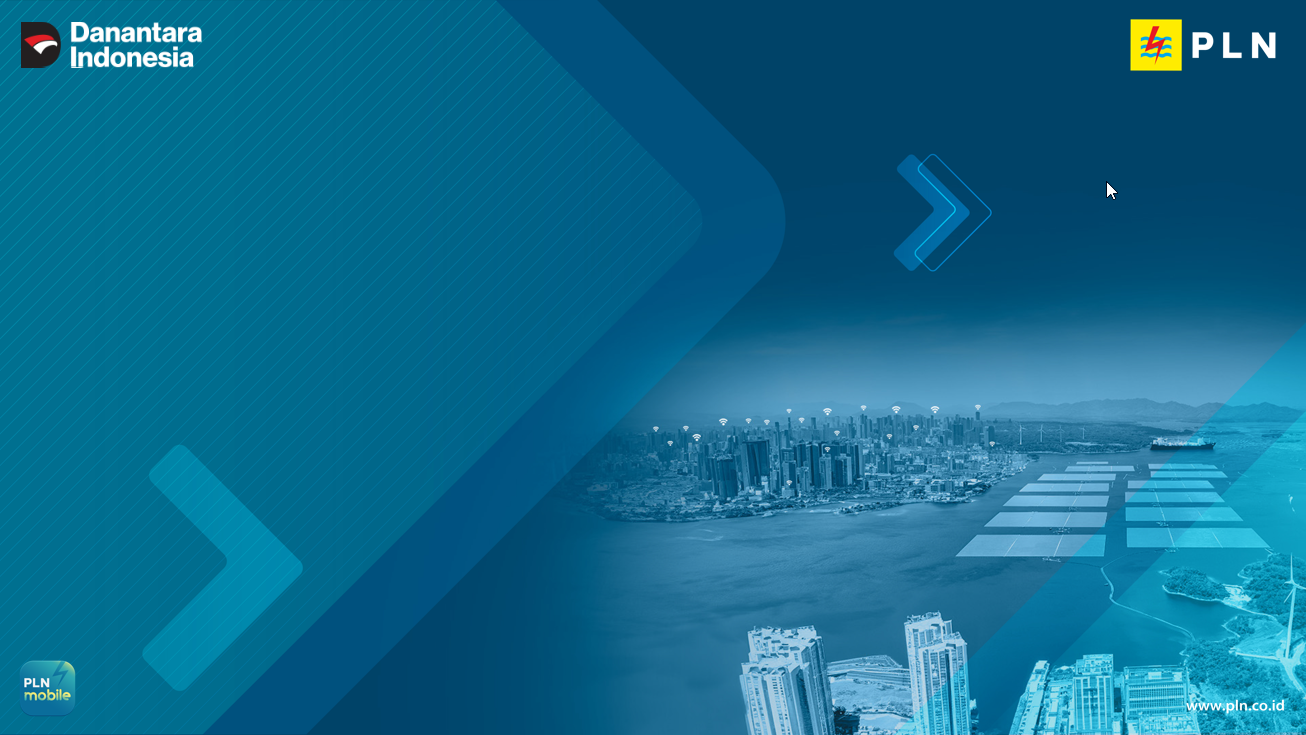
\includegraphics[width=\paperwidth,height=\paperheight]{assets/section.png}}
    \begin{frame}[plain]
      \vfill
      \centering
      {\Huge\bfseries\textcolor{white}{\insertsectionhead}\par}
      \vspace{0.5cm}
      {\large\textcolor{white!80}{Modul 4.4: Keamanan \& Keterlacakan Terintegrasi}\par}
      \vfill
    \end{frame}
  }
}

\begin{document}

% ================================================================
%  BAGIAN PEMBUKA
% ================================================================

% SLIDE 1: TITLE PAGE
{
\usebackgroundtemplate{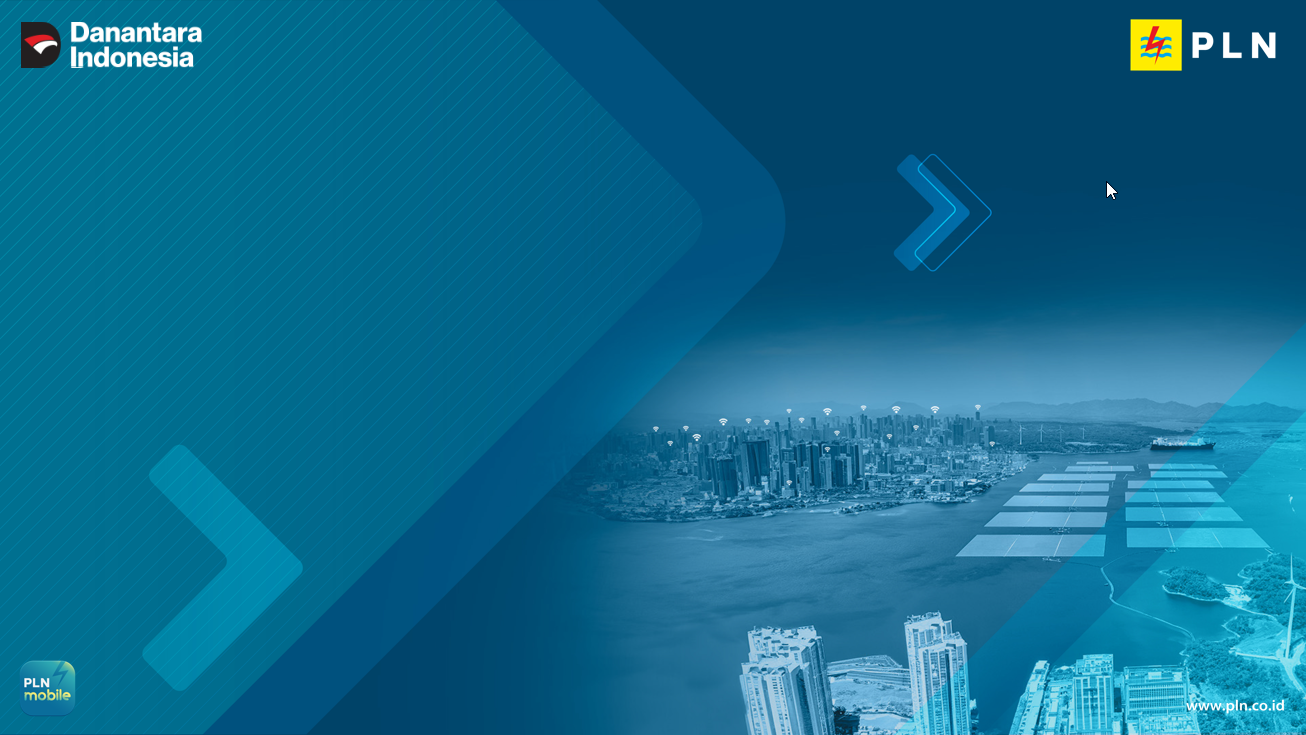
\includegraphics[width=\paperwidth,height=\paperheight]{assets/section.png}}
\setbeamercolor{title}{fg=white}
\setbeamercolor{author}{fg=white}
\setbeamercolor{institute}{fg=white}
\setbeamercolor{date}{fg=white}
\beamertemplatenavigationsymbolsempty
\begin{frame}[plain]
    \titlepage
\end{frame}
}

% SLIDE 2: SASARAN & PRASYARAT
\begin{frame}{Sasaran \& Prasyarat Peserta}
    \vspace{0.2cm}
    \begin{columns}[T]
        \column{0.48\textwidth}
        \begin{premiumbox}[Target Peserta]
            \small
            Modul ini ditujukan secara khusus bagi:
            \begin{itemize}
                \item \textbf{Manajemen Atas (MA)} PT PLN (Persero).
                \item Unit Kearsipan, IT Governance, GCG, Manajemen Risiko.
                \item Pengambil Kebijakan Tata Kelola Keamanan Informasi.
            \end{itemize}
        \end{premiumbox}
        
        \column{0.48\textwidth}
        \begin{orangebox}[Prasyarat Peserta]
            \scriptsize
            Untuk efektivitas pembelajaran, peserta diharapkan:
            \begin{itemize}
                \item Lulus \textbf{Modul 4.1--4.3} (arsitektur \& optimalisasi).
                \item Memahami klasifikasi arsip dasar \& familiar SSO/SAP.
                \item Membawa contoh kebijakan keamanan unit untuk studi kasus.
            \end{itemize}
        \end{orangebox}
    \end{columns}
\end{frame}

% SLIDE 3: TUJUAN PEMBELAJARAN
\begin{frame}{Tujuan Pembelajaran \& Target Kompetensi}
    \vspace{0.2cm}
    \begin{premiumbox}[Kompetensi Akhir Modul 4.4]
        \small
        Setelah menyelesaikan pelatihan ini, peserta ditargetkan mampu:
    \end{premiumbox}
    \vspace{0.3cm}
    \begin{columns}[T]
        \column{0.45\textwidth}
        \stepicon{plnblue}{1} \textbf{Merancang RBAC Terintegrasi}\\
        \vspace{0.1cm}
        \small
        Skema kontrol akses berbasis peran yang terhubung dengan sistem kepegawaian/SSO.
        \vspace{0.3cm}
        
        \stepicon{plncyan}{2} \textbf{Merancang Audit Trail}\\
        \vspace{0.1cm}
        \small
        Mekanisme log otomatis, 4W metadata, hash chain, \& SIEM.
        
        \column{0.48\textwidth}
        \stepicon{plnorange}{3} \textbf{Merumuskan Kebijakan ISMS}\\
        \vspace{0.1cm}
        \small
        Kebijakan keamanan arsip selaras ISO 27001, NIST, \& GCG BUMN.
        \vspace{0.3cm}
        
        \stepicon{plngreen}{4} \textbf{Merancang Backup \& DR}\\
        \vspace{0.1cm}
        \small
        Strategi 3-2-1, RTO/RPO, BCP, \& simulasi pemulihan.
    \end{columns}
\end{frame}

% SLIDE 4: AGENDA
\begin{frame}{Agenda Pembelajaran}
    \begin{columns}[T]
        \column{0.31\textwidth}
        \begin{tcolorbox}[colback=plnblue!5!white, colframe=plnblue, fonttitle=\bfseries\footnotesize, sharp corners, boxrule=0.6pt, left=2pt, right=2pt, top=0.5pt, bottom=0.5pt, title={Bagian I:\\Fondasi \& Urgensi}]
            \makebox[\linewidth][r]{%
                \tcbox[on line, colback=plnblue!15, colframe=plnblue, boxrule=0.5pt, arc=2pt, boxsep=0pt, left=2pt, right=2pt, top=0.5pt, bottom=0.5pt, fontupper=\bfseries\tiny\color{plnblue}]{5 menit}%
            }
            \scriptsize
            \stepicon{plnblue}{1} \textbf{Konteks \& Urgensi}\\
            {\tiny Serangan siber, regulasi, GCG.}\\
            \stepicon{plnblue}{2} \textbf{Arsitektur 4 Pilar}\\
            {\tiny RBAC, Audit, ISMS, Backup/DR.}
        \end{tcolorbox}
        
        \column{0.31\textwidth}
        \begin{tcolorbox}[colback=plnorange!5!white, colframe=plnorange, fonttitle=\bfseries\footnotesize, sharp corners, boxrule=0.6pt, left=2pt, right=2pt, top=0.5pt, bottom=0.5pt, title={Bagian II:\\Empat Pilar Keamanan}]
            \makebox[\linewidth][r]{%
                \tcbox[on line, colback=plnorange!15, colframe=plnorange, boxrule=0.5pt, arc=2pt, boxsep=0pt, left=2pt, right=2pt, top=0.5pt, bottom=0.5pt, fontupper=\bfseries\tiny\color{plnorange}]{37 menit}%
            }
            \scriptsize
            \stepicon{plnorange}{3} \textbf{Pilar 1: RBAC}\\
            \stepicon{plnorange}{4} \textbf{Pilar 2: Audit Trail}\\
            \stepicon{plnorange}{5} \textbf{Pilar 3: Kebijakan ISMS}\\
            \stepicon{plnorange}{6} \textbf{Pilar 4: Backup \& DR}
        \end{tcolorbox}
        
        \column{0.31\textwidth}
        \begin{tcolorbox}[colback=plngreen!5!white, colframe=plngreen, fonttitle=\bfseries\footnotesize, sharp corners, boxrule=0.6pt, left=2pt, right=2pt, top=0.5pt, bottom=0.5pt, title={Bagian III:\\Studi Kasus \& Validasi}]
            \makebox[\linewidth][r]{%
                \tcbox[on line, colback=plngreen!15, colframe=plngreen, boxrule=0.5pt, arc=2pt, boxsep=0pt, left=2pt, right=2pt, top=0.5pt, bottom=0.5pt, fontupper=\bfseries\tiny\color{plngreen}]{3 menit}%
            }
            \scriptsize
            \stepicon{plngreen}{7} \textbf{Studi Kasus Integratif}\\
            {\tiny Insiden kebocoran arsip.}\\
            \stepicon{plngreen}{8} \textbf{Portofolio \& Kendali Manajemen}\\
            {\tiny Rubrik, komitmen, tindak lanjut.}
        \end{tcolorbox}
    \end{columns}
    \centering
    \vspace{0.15cm}
    \textcolor{darkgrey}{\scriptsize \textit{Durasi fasilitasi: 45 menit (Fondasi 5$\cdot$ RBAC 10$\cdot$ Audit 10$\cdot$ ISMS 10$\cdot$ DR 7$\cdot$ Kasus 3), workshop mandiri 4$\times$30 menit}}
\end{frame}

% SLIDE 5: KONTEKS & URGENSI
\begin{frame}{Konteks \& Urgensi: Mengapa Ini Penting bagi PLN?}
    \vspace{0.2cm}
    \begin{columns}[T]
        \column{0.55\textwidth}
        \begin{orangebox}[Ancaman yang Terus Meningkat]
            \scriptsize
            \begin{itemize}
                \item \textbf{2021:} 1,63 miliar anomali serangan siber (BSSN).
                \item \textbf{Jan--Jul 2025:} 3,64 miliar anomali --- BUMN jadi target utama.
                \item Kebocoran kontrak strategis = kerugian finansial + sanksi regulasi.
            \end{itemize}
        \end{orangebox}
        \begin{premiumbox}[Risiko Ganda]
            \scriptsize
            \begin{enumerate}
                \item \textbf{Operasional:} Kehilangan aset informasi kritis.
                \item \textbf{Regulasi:} Sanksi OJK, BPK, ANRI, temuan audit.
            \end{enumerate}
        \end{premiumbox}
        
        \column{0.43\textwidth}
        \begin{greenbox}[Implikasi GCG]
            \scriptsize
            Kegagalan menjaga keamanan arsip langsung memengaruhi penilaian \textbf{TARIF} BUMN:
            \begin{itemize}
                \scriptsize
                \item \textbf{Transparansi} audit trail
                \item \textbf{Akuntabilitas} keputusan
                \item \textbf{Responsibilitas} kepatuhan
            \end{itemize}
        \end{greenbox}
    \end{columns}
\end{frame}

% SLIDE 6: ARSITEKTUR 4 PILAR
\begin{frame}{Arsitektur Keamanan Terintegrasi: 4 Pilar}
    \vspace{0.2cm}
    \centering
    \begin{tikzpicture}[
        arrp/.style={-{Stealth[length=6pt]}, thick, color=gray!50}
    ]
        \node[pilar=plnblue] (p1) at (0,0) {PILAR 1\\RBAC\\Kontrol Akses};
        \node[pilar=plncyan] (p2) at (4,0) {PILAR 2\\Audit Trail\\Keterlacakan};
        \node[pilar=plnorange] (p3) at (8,0) {PILAR 3\\Kebijakan\\ISMS};
        \node[pilar=plngreen] (p4) at (12,0) {PILAR 4\\Backup/DR\\Ketersediaan};
        
        \draw[arrp] (p1) -- (p2);
        \draw[arrp] (p2) -- (p3);
        \draw[arrp] (p3) -- (p4);
        
        \node[font=\tiny, text=gray] at (0,1.3) {WHO?};
        \node[font=\tiny, text=gray] at (4,1.3) {WHEN/WHAT?};
        \node[font=\tiny, text=gray] at (8,1.3) {HOW?};
        \node[font=\tiny, text=gray] at (12,1.3) {HOW?};
    \end{tikzpicture}
    
    \vspace{0.4cm}/
    \begin{premiumbox}[Pandangan Strategis]
        \small
        Keempat pilar harus dirancang \textbf{bersamaan}, bukan berurutan oleh unit yang berbeda tanpa koordinasi. Solusi parsial = celah keamanan yang tidak terdeteksi hingga terjadi insiden.
    \end{premiumbox}
\end{frame}

% SLIDE 7: KERANGKA BERPIKIR
\begin{frame}{Kerangka Berpikir Modul 4.4}
    \centering
    \begin{columns}
        \column{0.55\textwidth}
        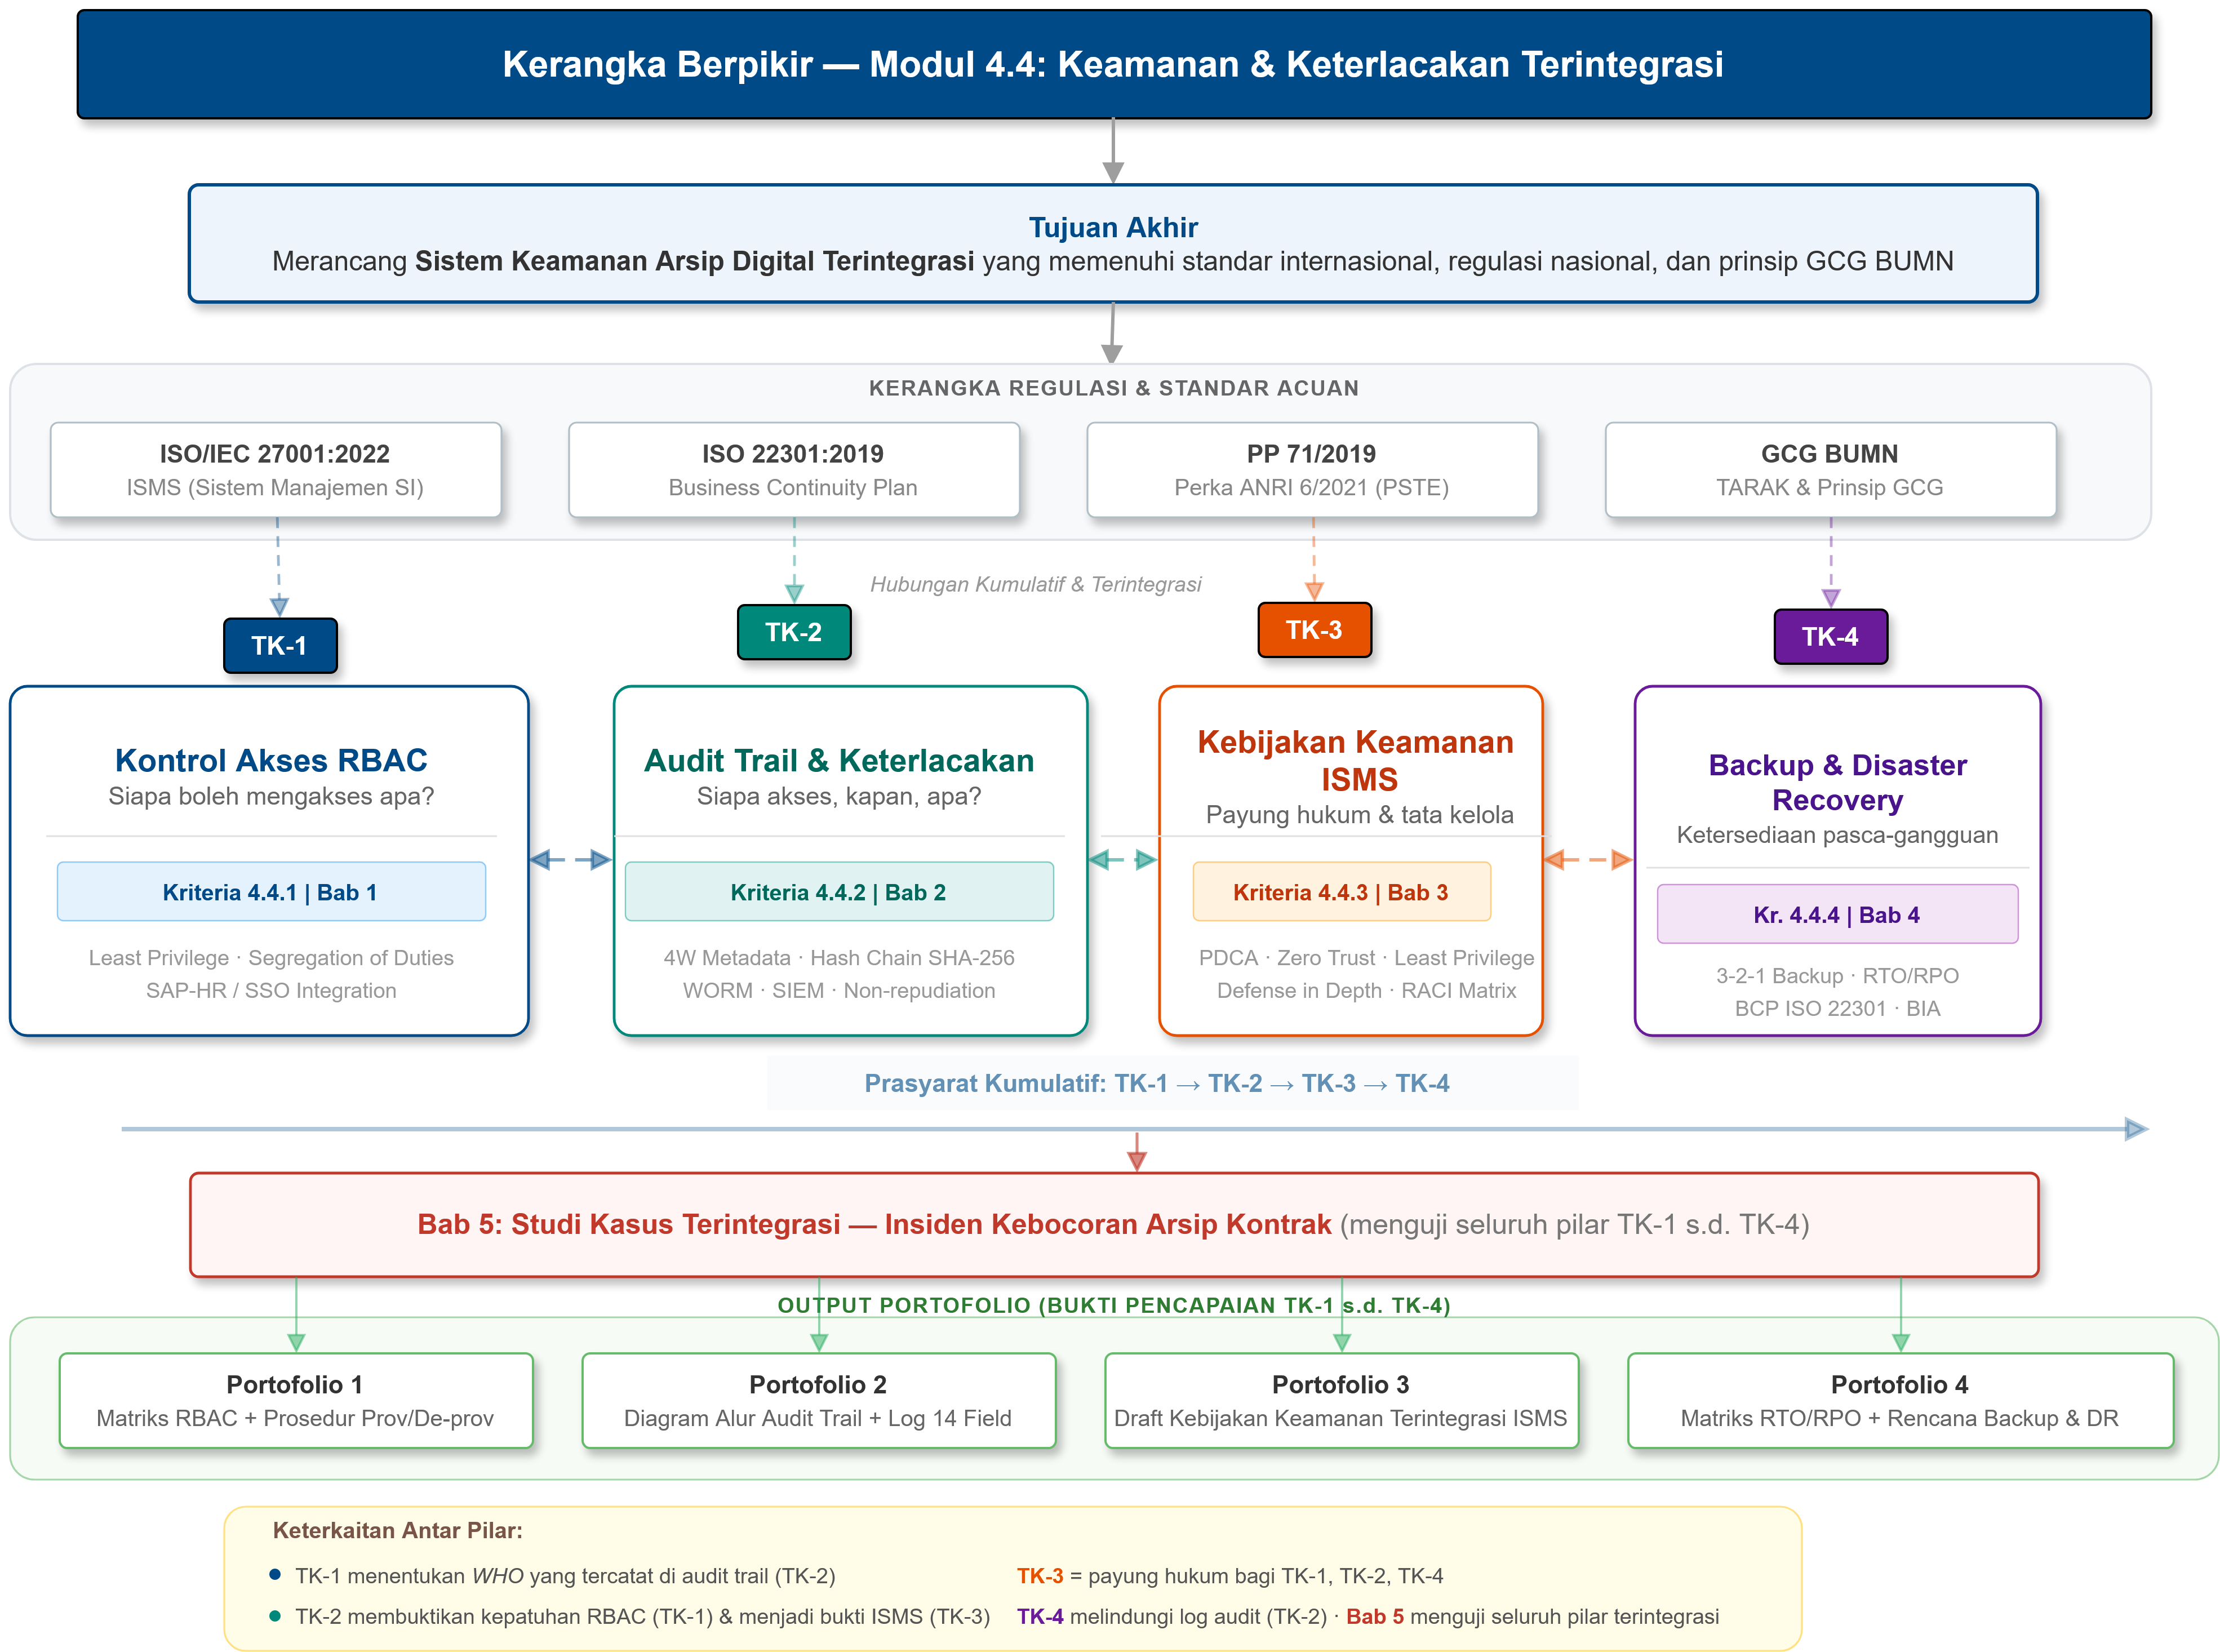
\includegraphics[width=\linewidth,keepaspectratio]{gambar/kerangka_pikir.png}
        
        \column{0.43\textwidth}
        \scriptsize
        \begin{premiumbox}[Peta Jalan Kompetensi]
            \begin{itemize}
                \item \textbf{TK-1 (Bab 1):} Siapa yang boleh mengakses?
                \item \textbf{TK-2 (Bab 2):} Kapan \& apa yang dilakukan?
                \item \textbf{TK-3 (Bab 3):} Payung hukum \& tata kelola.
                \item \textbf{TK-4 (Bab 4):} Jamin ketersediaan pasca-gangguan.
            \end{itemize}
        \end{premiumbox}
        \vspace{0.1cm}
        \begin{orangebox}[Puncak Pembelajaran]
            Studi Kasus Bab 5 menguji apakah keempat pilar diterapkan secara sinergis.
        \end{orangebox}
    \end{columns}
\end{frame}


% ================================================================
%  BAGIAN I: PILAR 1 -- RBAC
% ================================================================

\section{Pilar 1:\\Kontrol Akses Berbasis Peran (RBAC)}

% SLIDE 8: PRINSIP RBAC
\begin{frame}{Tiga Prinsip Fundamental RBAC}
    \vspace{0.2cm}
    \begin{columns}[T]
        \column{0.31\textwidth}
        \centering
        \stepicon{plnblue}{1} \\ \textbf{Least Privilege} \\
        \vspace{0.1cm}
        \scriptsize Hak akses minimum yang benar-benar diperlukan. Staf TU tidak perlu hak Export terhadap arsip Rahasia jika tugasnya hanya Read.
        
        \column{0.31\textwidth}
        \centering
        \stepicon{plncyan}{2} \\ \textbf{Segregation of Duties} \\
        \vspace{0.1cm}
        \scriptsize Tidak ada satu peran yang memiliki kombinasi hak berlebihan: Create, Approve, \& Export harus terpisah.
        
        \column{0.31\textwidth}
        \centering
        \stepicon{plnorange}{3} \\ \textbf{Break-Glass} \\
        \vspace{0.1cm}
        \scriptsize Akses darurat di luar hak normal, dengan pencatatan audit trail lengkap \& persetujuan atasan pasca-kejadian.
    \end{columns}
    
    \vspace{0.4cm}
    \begin{premiumbox}[Mengapa RBAC = Fondasi Keterlacakan?]
        \small
        Tanpa kontrol akses terstruktur, log audit menjadi tidak bermakna. RBAC memastikan setiap jejak digital merepresentasikan tindakan pihak yang \textbf{berwenang}.
    \end{premiumbox}
\end{frame}

% SLIDE 9: MODEL RBAC NIST
\begin{frame}{Model RBAC NIST}
    \centering
    \resizebox{0.85\textwidth}{!}{%
    \begin{tikzpicture}[
      box/.style={draw=plnblue, fill=plnblue!5, rounded corners=4pt,
        line width=0.8pt, minimum width=2.8cm, minimum height=1.4cm,
        font=\small, align=center},
      arr/.style={-{Stealth[length=5pt]}, line width=0.7pt, plnblue},
      lbl/.style={font=\tiny, fill=white, inner sep=2pt, text=plnblue!80!black}
    ]
    \node[box] (users) at (0,3) {\textbf{USERS}\\[-1pt]{\scriptsize Pengguna PLN}};
    \node[box] (roles) at (5,3) {\textbf{ROLES}\\[-1pt]{\scriptsize Jabatan / Peran}};
    \node[box] (perms) at (10,3) {\textbf{PERMISSIONS}\\[-1pt]{\scriptsize Hak Akses}};
    \node[box] (sess)  at (2.5,0) {\textbf{SESSIONS}\\[-1pt]{\scriptsize Sesi Aktif}};
    \draw[arr] (users) -- node[lbl, above]{UA} (roles);
    \draw[arr] (roles) -- node[lbl, above]{PA} (perms);
    \draw[arr] (users.south) -- node[lbl, left]{SC} (sess.north west);
    \draw[arr] (sess.east) -- node[lbl, below, sloped]{SA} (roles.south);
    \end{tikzpicture}%
    }
    
    \vspace{0.3cm}
    \begin{orangebox}[Insight]
        \small
        Hak akses tidak diberikan langsung ke individu, melainkan ke \textbf{peran} (role). Pendekatan ini mempermudah manajemen siklus hidup akses: provisioning saat mutasi \& de-provisioning saat pensiun.
    \end{orangebox}
\end{frame}

% SLIDE 10: MATRIKS RBAC
\begin{frame}{Matriks RBAC: Role $\times$ Klasifikasi Arsip PLN}
    \vspace{0.1cm}
    \centering
    \scriptsize
    \begin{tabularx}{\textwidth}{@{} >{\raggedright\arraybackslash}p{2.6cm} >{\centering\arraybackslash}p{1.8cm} >{\centering\arraybackslash}p{1.8cm} >{\centering\arraybackslash}p{1.8cm} >{\centering\arraybackslash}p{1.8cm} @{}}
        \toprule
        \rowcolor{rowhead}
        \textcolor{white}{\textbf{Peran}} & \textcolor{white}{\textbf{Publik}} & \textcolor{white}{\textbf{Terbatas}} & \textcolor{white}{\textbf{Rahasia}} & \textcolor{white}{\textbf{Vital}} \\
        \midrule
        \rowcolor{rowalt}
        Staf Kearsipan & C, R & R & R$^{\dagger}$ & -- \\
        Staf Administrasi/TU & C, R & R & -- & -- \\
        \rowcolor{rowalt}
        Kabag TU / Kasubag & C, R, U & C, R, U & R, E & R \\
        Staf Hukum / Legal & C, R & C, R, U & R, E & R \\
        \rowcolor{rowalt}
        Staf IT / DBA & -- & R & R & R$^{\dagger}$ \\
        GM / SRM Unit & R & R, U & R, U, A & R, U, A \\
        \rowcolor{rowalt}
        Auditor SPI & R & R, E & R, E & R, E \\
        VP Cyber Security & R & R, E & R, E & R, E \\
        \bottomrule
    \end{tabularx}
    
    \vspace{0.1cm}
    {\tiny C=Create, R=Read, U=Update, A=Approve, E=Export/Review. $^{\dagger}$Dengan persetujuan atasan.}
    
    \vspace{0.1cm}
    \begin{greenbox}[Arah Manajemen Atas]
        \scriptsize Validasi: tidak ada satu peran yang sekaligus Create, Approve, \& Export arsip Vital tanpa mekanisme pengawasan.
    \end{greenbox}
\end{frame}

% SLIDE 11: LANGKAH PERANCANGAN RBAC
\begin{frame}{Langkah Perancangan Skema RBAC}
    \vspace{0.2cm}
    \begin{columns}[T]
        \column{0.48\textwidth}
        \begin{premiumbox}[Tata Kelola bagi MA]
            \scriptsize
            \begin{enumerate}
                \item \textbf{Inventarisasi Peran} -- Validasi kelengkapan daftar peran.
                \item \textbf{Pemetaan Aset} -- Tetapkan klasifikasi 4 tingkat (Vital, Rahasia, Terbatas, Publik).
                \item \textbf{Penetapan Hak Minimum} -- Tim IT + Kearsipan susun matriks; MA setujui.
            \end{enumerate}
        \end{premiumbox}
        
        \column{0.48\textwidth}
        \begin{orangebox}[Validasi Kritis]
            \scriptsize
            \begin{enumerate}\setcounter{enumi}{3}
                \item \textbf{Segregation of Duties} -- Pastikan tidak ada konflik kepentingan.
                \item \textbf{Provisioning/De-provisioning} -- Terhubung SAP-HR/SSO.
                \item \textbf{Review Berkala} -- Minimal tahunan, hasilnya didokumentasikan.
            \end{enumerate}
        \end{orangebox}
    \end{columns}
    
    \vspace{0.2cm}
    \begin{center}
        \textcolor{plnblue}{\scriptsize\textit{Pertanyaan Kunci: ``Apakah hak akses langsung dicabut saat mutasi/pensiun tanpa menunggu keluhan?''}}
    \end{center}
\end{frame}

% SLIDE 12: OUTPUT PILAR 1
\begin{frame}{Output \& Workshop: Pilar 1 (RBAC)}
    \vspace{0.2cm}
    \begin{columns}[T]
        \column{0.48\textwidth}
        \begin{premiumbox}[Workshop 1 (30 Menit)]
            \scriptsize
            \begin{enumerate}
                \item Identifikasi 3 peran kunci di unit Anda yang bersentuhan dengan arsip.
                \item Tentukan hak akses (CRU) untuk 3 klasifikasi arsip operasional.
                \item Rancang mekanisme review \& revokasi akses tahunan.
            \end{enumerate}
        \end{premiumbox}
        
        \column{0.48\textwidth}
        \begin{greenbox}[Portofolio 1]
            \scriptsize
            \textbf{Matriks RBAC Terintegrasi} + Prosedur Provisioning/De-provisioning.\\[0.1cm]
            \textit{Kriteria:} 4.4.1 -- kejelasan role, least privilege, integrasi HR/SSO.
        \end{greenbox}
    \end{columns}
\end{frame}

% ================================================================
%  BAGIAN II: PILAR 2 -- AUDIT TRAIL
% ================================================================

\section{Pilar 2:\\Audit Trail Otomatis \& Keterlacakan}

% SLIDE 13: KONSEP AUDIT TRAIL
\begin{frame}{Mengapa Audit Trail Berurutan setelah RBAC?}
    \vspace{0.2cm}
    \begin{premiumbox}[Analogi]
        \small
        RBAC mengontrol siapa yang boleh masuk pintu. Audit trail adalah \textbf{kamera CCTV} yang merekam setiap orang yang masuk, kapan, dan melakukan apa.
    \end{premiumbox}
    
    \begin{columns}[T]
        \column{0.48\textwidth}
        \begin{orangebox}[SIEM]
            \scriptsize
            \textbf{Security Information \& Event Management} -- ``kamera pengawas digital'' yang mengubah ribuan log mentah menjadi informasi yang dapat ditindaklanjuti secara proaktif.
        \end{orangebox}
        
        \column{0.48\textwidth}
        \begin{greenbox}[Hash Chain]
            \scriptsize
            Setiap entri log dihubungkan secara kriptografis. Jika 1 byte diubah, seluruh rantai hash berikutnya \textbf{gagal verifikasi} --- manipulasi langsung terdeteksi.
        \end{greenbox}
    \end{columns}
\end{frame}

% SLIDE 14: DIAGRAM ALUR AUDIT TRAIL
\begin{frame}{Diagram Alur Audit Trail Sistem Arsip Digital PLN}
    \centering
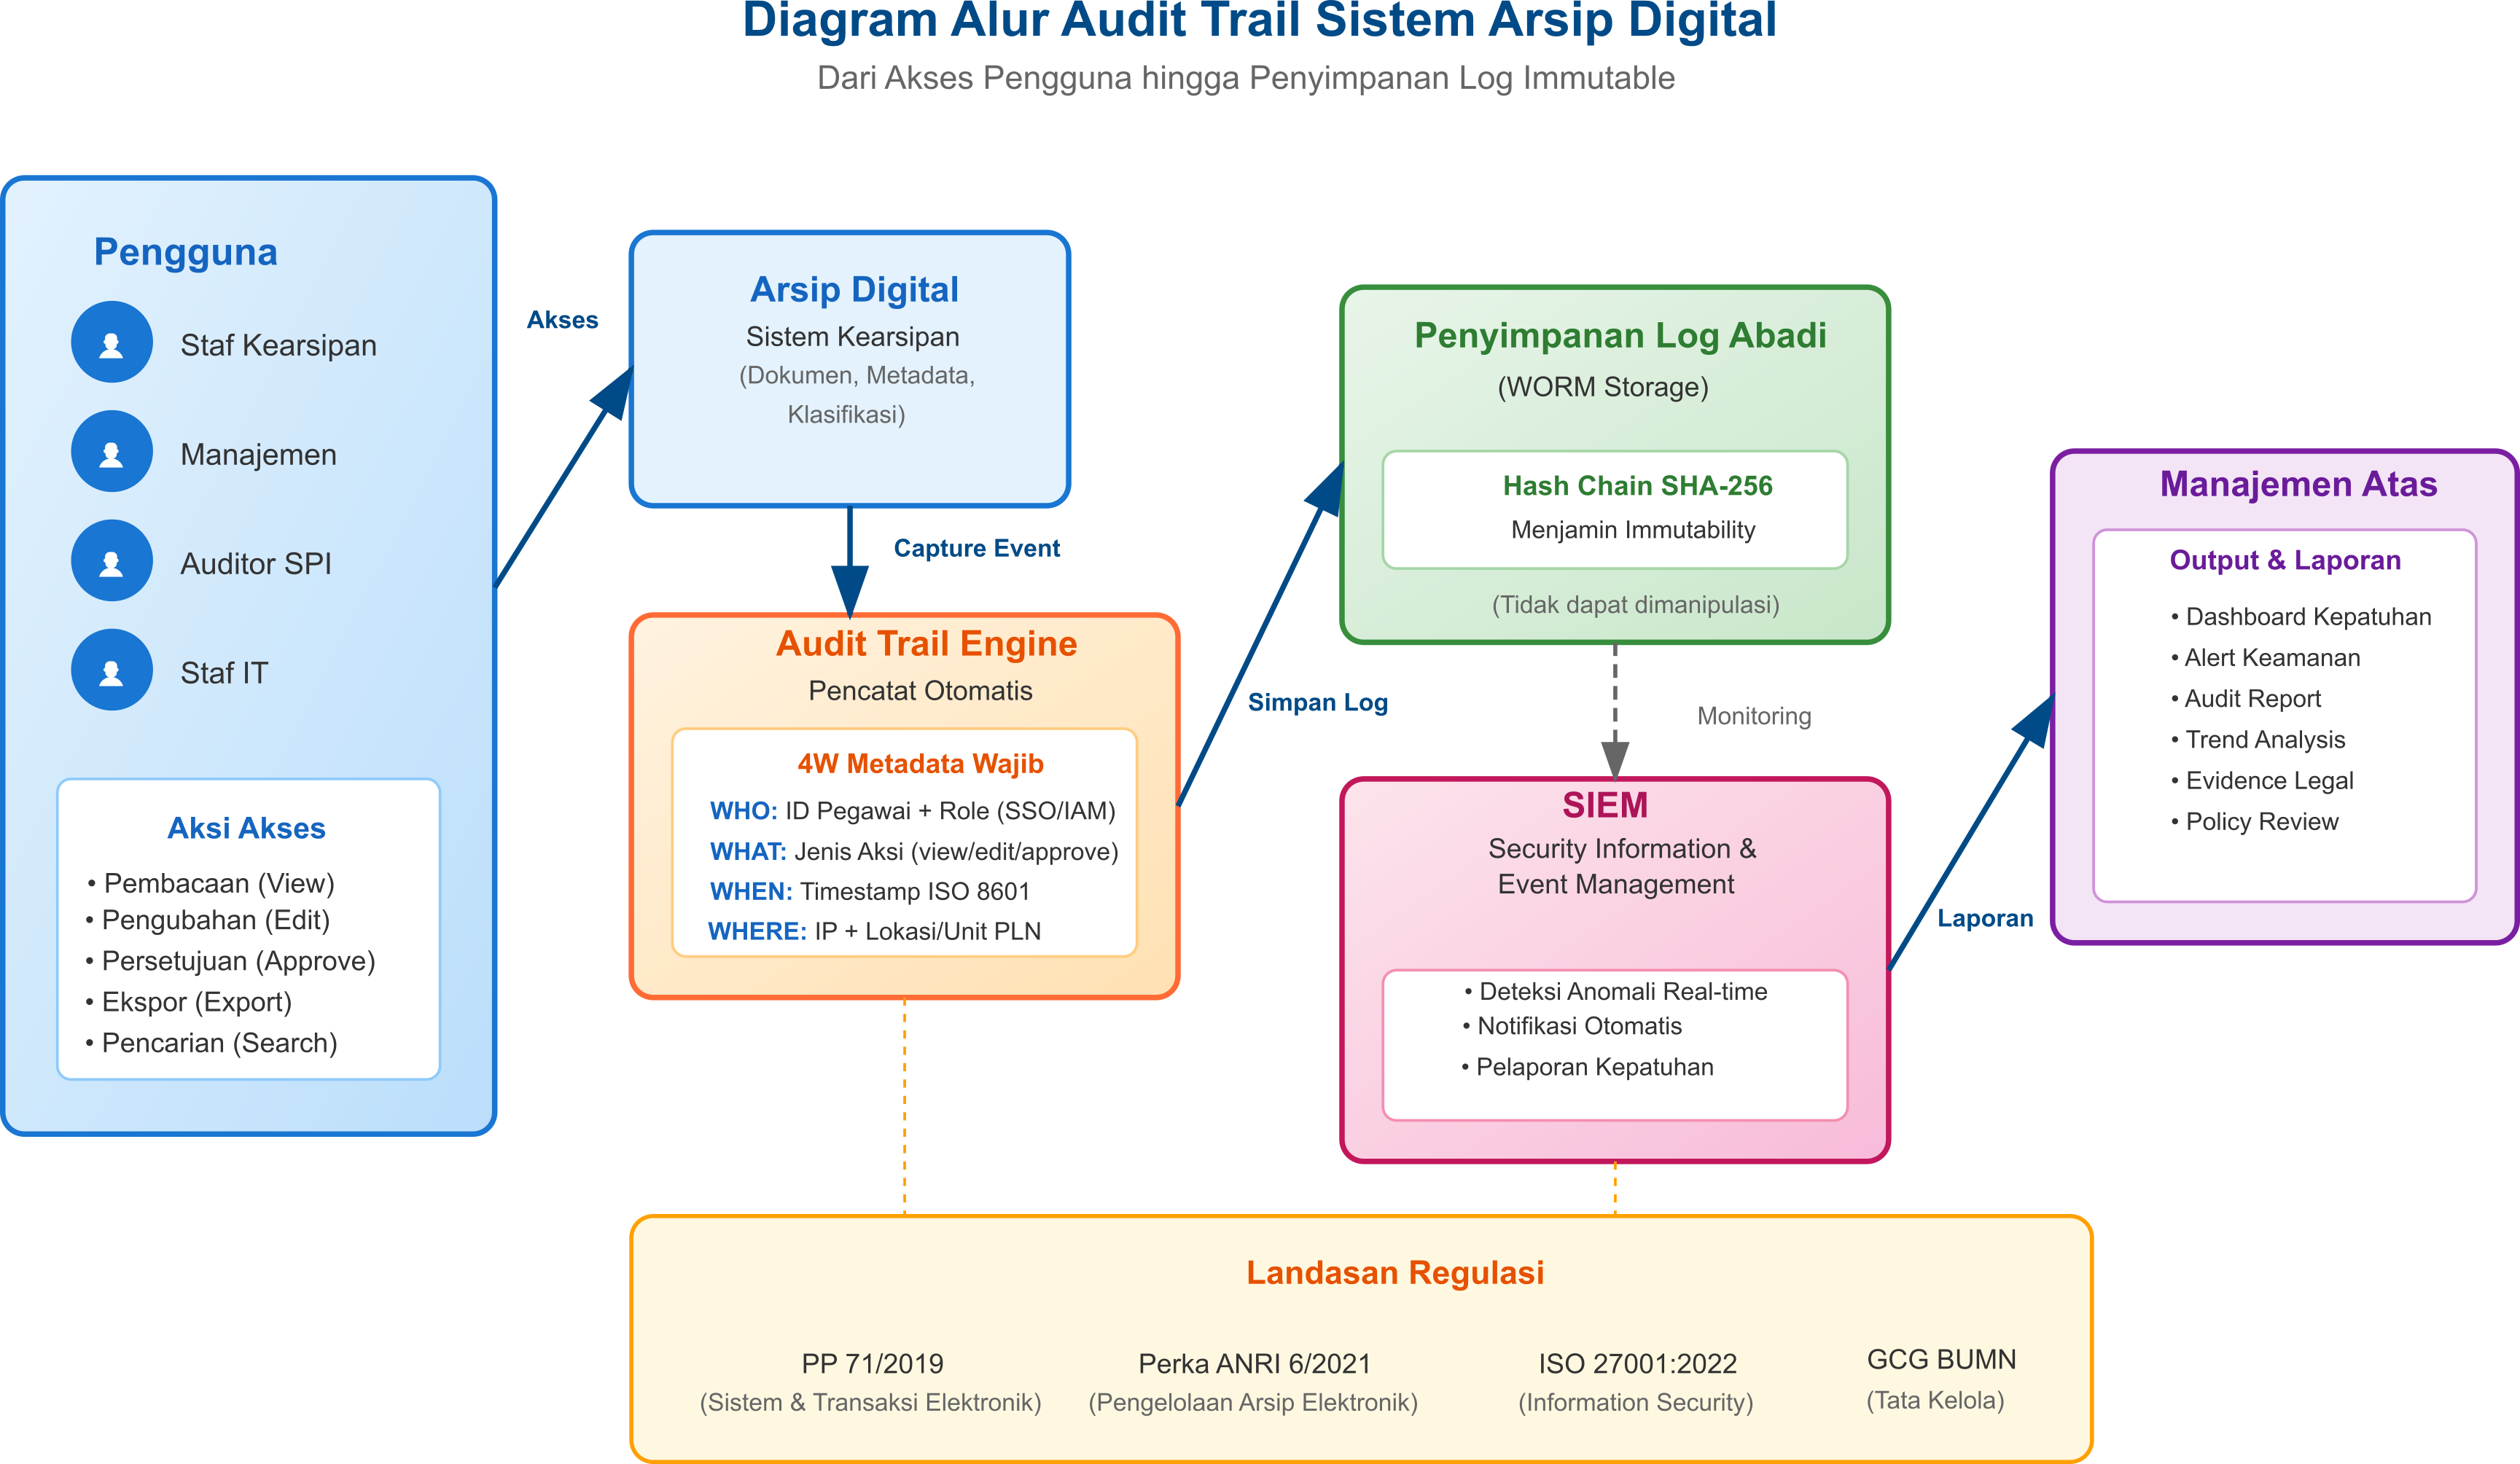
\includegraphics[width=0.60\textwidth,keepaspectratio]{audit_v3.png}
    \vspace{0.6cm}
    {\centering
    \begin{tabular}{@{} >{\centering\arraybackslash\tiny}p{1.8cm} >{\centering\arraybackslash\tiny}p{1.7cm} >{\centering\arraybackslash\tiny}p{1.4cm} >{\centering\arraybackslash\tiny}p{1.3cm} @{}}
        \toprule
        \textbf{WHO} & \textbf{WHAT} & \textbf{WHEN} & \textbf{WHERE} \\
        \midrule
        ID Pegawai + Role (SSO) & Aksi: view/edit/export & Timestamp ISO 8601 & IP + Lokasi Unit \\
        \bottomrule
    \end{tabular}
    \par}
\end{frame}

% SLIDE 15: 14 FIELD METADATA
\begin{frame}{14 Field Metadata Audit Trail}
    \vspace{0.2cm}
    \begin{columns}[T]
        \column{0.48\textwidth}
        \begin{premiumbox}[Wajib (12 Field)]
            \tiny
            \begin{itemize}
                \item \texttt{DOC\_ID} -- ID Dokumen Unik
                \item \texttt{TIMESTAMP} -- Waktu Aksi (ISO 8601)
                \item \texttt{HASH\_SHA256} -- Nilai Hash Integritas
                \item \texttt{CREATOR\_ROLE} -- Peran Pengguna (IAM/SSO)
                \item \texttt{AUDIT\_LOG\_ID} -- ID Log Immutable
                \item \texttt{CLASSIFICATION} -- Tingkat Keamanan
                \item \texttt{RETENTION\_RULE} -- Aturan Retensi
                \item \texttt{ASSET\_ID} -- Referensi Aset PLN
                \item \texttt{CONTRACT\_REF} -- Referensi Kontrak
                \item \texttt{LOCATION\_GIS} -- Lokasi Operasional
                \item \texttt{INTEGRITY\_HASH} -- Verifikasi Perubahan
                \item \texttt{AUDIT\_TRAIL\_REF} -- Log Terkait
            \end{itemize}
        \end{premiumbox}
        
        \column{0.48\textwidth}
        \begin{orangebox}[Semi-Mandatory (2 Field)]
            \tiny
            \begin{itemize}
                \item \texttt{CONTENT\_DESC} -- Ringkasan Isi (NLP/Input)
                \item \texttt{SEARCH\_TAGS} -- Kata Kunci Terkontrol
            \end{itemize}
        \end{orangebox}
        \vspace{0.1cm}
        \begin{greenbox}[Regulasi]
            \scriptsize Memenuhi PP 71/2019 \& Perka ANRI 6/2021.
        \end{greenbox}
    \end{columns}
\end{frame}

% SLIDE 16: HASH CHAIN
\begin{frame}{Hash Chain: Immutability Log Audit}
    \centering
    \resizebox{0.75\textwidth}{!}{%
    \begin{tikzpicture}[
      ok/.style={draw=plnblue, fill=plnblue!5, rounded corners=2pt,
        line width=0.5pt, minimum width=1.2cm, minimum height=1.3cm,
        align=center, font=\tiny, inner sep=2pt},
      fail/.style={draw=red!70!black, fill=red!5, rounded corners=2pt,
        line width=0.5pt, minimum width=1.2cm, minimum height=1.3cm,
        align=center, font=\tiny, inner sep=2pt},
      warn/.style={draw=orange!80!black, fill=orange!5, rounded corners=2pt,
        line width=0.5pt, minimum width=1.2cm, minimum height=1.3cm,
        align=center, font=\tiny, inner sep=2pt},
      arr/.style={-{Stealth[length=2pt]}, line width=0.5pt}
    ]
    \node[font=\tiny\bfseries, text=plnblue] at (5,3.8)
      {Hash Chain: Immutability Log Audit};
    \node[font=\tiny, text=gray] at (5,3.4)
      {Modifikasi 1 byte merusak rantai};
    \node[ok] (L1) at (0,1.5) {\textbf{Log 1}\\[-1pt]{\tiny a4f8c2}\\
      {\tiny 08:30}\\[-1pt]{\tiny\color{green!60!black}$\checkmark$}};
    \node[ok] (L2) at (2.5,1.5) {\textbf{Log 2}\\[-1pt]{\tiny 7d3e91}\\
      {\tiny 09:15}\\[-1pt]{\tiny\color{green!60!black}$\checkmark$}};
    \node[fail] (L3) at (5,1.5) {\textbf{Log 3}\\[-1pt]{\tiny\color{red!70!black}3b6c45}\\
      {\tiny 23:45}\\[-1pt]{\tiny\color{red!70!black}$\times$}};
    \node[warn] (L4) at (7.5,1.5) {\textbf{Log 4}\\[-1pt]{\tiny b1c7f3}\\
      {\tiny 10:00}\\[-1pt]{\tiny\color{orange!80!black}$\times$}};
    \node[warn] (L5) at (10,1.5) {\textbf{Log 5}\\[-1pt]{\tiny e9d4a6}\\
      {\tiny 14:30}\\[-1pt]{\tiny\color{orange!80!black}$\times$}};
    \draw[arr, plnblue] (L1) -- (L2);
    \draw[arr, red!70!black] (L2) -- (L3);
    \draw[arr, orange!80!black] (L3) -- (L4);
    \draw[arr, orange!80!black] (L4) -- (L5);
    \node[font=\tiny\bfseries, text=red!70!black] at (5,-0.3)
      {INTEGRITAS TERDETEKSI RUSAK};
    \end{tikzpicture}%
    }
    
    \vspace{0.2cm}
    \begin{premiumbox}[Pesan untuk MA]
        \small
        Hash SHA-256 menjamin deteksi perubahan 1 byte seketika. Log disimpan terpisah (WORM). Setiap approval wajib \textbf{TTE} untuk kekuatan hukum non-repudiation.
    \end{premiumbox}
\end{frame}

% SLIDE 17: LANGKAH PERANCANGAN AUDIT TRAIL
\begin{frame}{Langkah Perancangan Audit Trail}
    \vspace{0.2cm}
    \begin{columns}[T]
        \column{0.48\textwidth}
        \begin{premiumbox}[Tata Kelola]
            \scriptsize
            \begin{enumerate}
                \item \textbf{Cakupan \& Retensi} -- Minimal arsip Rahasia/Vital; retensi = masa retensi arsip.
                \item \textbf{Validasi Metadata} -- Pastikan 14 field tercatat; minta bukti laporan log.
                \item \textbf{Mekanisme Pemantauan} -- SIEM: mingguan (Vital), bulanan (Rahasia).
            \end{enumerate}
        \end{premiumbox}
        
        \column{0.48\textwidth}
        \begin{orangebox}[Eskalasi \& Kepatuhan]
            \scriptsize
            \begin{enumerate}\setcounter{enumi}{3}
                \item \textbf{Eskalasi} -- Siapa dihubungi dalam 1 jam / 4 jam / 24 jam?
                \item \textbf{Kepatuhan Regulasi} -- PP 71/2019 \& Perka ANRI 6/2021.
            \end{enumerate}
        \end{orangebox}
    \end{columns}
    
    \vspace{0.2cm}
    \begin{center}
        \textcolor{plnblue}{\scriptsize\textit{Pertanyaan Kunci: ``Jika hari ini terjadi kebocoran, bisakah kita tunjukkan siapa yang mengakses dalam 6 bulan terakhir?''}}
    \end{center}
\end{frame}

% SLIDE 18: OUTPUT PILAR 2
\begin{frame}{Output \& Workshop: Pilar 2 (Audit Trail)}
    \vspace{0.2cm}
    \begin{columns}[T]
        \column{0.48\textwidth}
        \begin{premiumbox}[Workshop 2 (30 Menit)]
            \scriptsize
            \begin{enumerate}
                \item Gambar alur audit trail: penciptaan $\rightarrow$ validasi $\rightarrow$ penyimpanan.
                \item Lengkapi template 14 field untuk 1 jenis arsip kritis.
                \item Tentukan mekanisme eskalasi jika hash integrity gagal.
            \end{enumerate}
        \end{premiumbox}
        
        \column{0.48\textwidth}
        \begin{greenbox}[Portofolio 2]
            \scriptsize
            \textbf{Diagram Alur Audit Trail} + Template Log 14 Field.\\[0.1cm]
            \textit{Kriteria:} 4.4.2 -- kelengkapan 4W, immutability, compliance regulasi.
        \end{greenbox}
    \end{columns}
\end{frame}


% ================================================================
%  BAGIAN III: PILAR 3 -- KEBIJAKAN ISMS
% ================================================================

\section{Pilar 3:\\Kebijakan Keamanan Terintegrasi dengan ISMS}

% SLIDE 19: MENGAPA KEBIJAKAN?
\begin{frame}{Mengapa Kebijakan Berurutan setelah RBAC \& Audit Trail?}
    \vspace{0.2cm}
    \begin{premiumbox}[Analogi]
        \small
        RBAC = Pintu \& Kunci. Audit Trail = CCTV. Kebijakan = \textbf{Peraturan Perusahaan} yang memberikan kekuatan hukum agar pintu tidak dibuka sembarangan dan CCTV tidak dimatikan.
    \end{premiumbox}
    
    \begin{columns}[T]
        \column{0.48\textwidth}
        \begin{orangebox}[ISO/IEC 27001:2022]
            \scriptsize
            93 kontrol keamanan dalam 4 kelompok: Organizational, People, Physical, Technological. Arsip digital = Aset Informasi Kritis.
        \end{orangebox}
        
        \column{0.48\textwidth}
        \begin{greenbox}[NIST]
            \scriptsize
            Cybersecurity Framework, SP 800-53, SP 800-207 (Zero Trust). Referensi praktikal global untuk perancangan kebijakan.
        \end{greenbox}
    \end{columns}
\end{frame}

% SLIDE 20: SIKLUS PDCA
\begin{frame}{Siklus PDCA: Fondasi ISO 27001}
    \centering
    \begin{columns}
        \column{0.45\textwidth}
        \resizebox{0.85\textwidth}{!}{%
        \begin{tikzpicture}
        \node[box2=plnblue]   (plan)  at (-2, 1.5) {\textbf{\color{plnblue}PLAN}\\[-1pt]
          {\scriptsize Kebijakan \& Risiko}};
        \node[box2=green!50!black] (do)    at ( 2, 1.5) {\textbf{\color{green!50!black}DO}\\[-1pt]
          {\scriptsize Implementasi Kontrol}};
        \node[box2=orange!80!black] (check) at ( 2,-1.5) {\textbf{\color{orange!80!black}CHECK}\\[-1pt]
          {\scriptsize Audit \& Evaluasi}};
        \node[box2=red!70!black]   (act)   at (-2,-1.5) {\textbf{\color{red!70!black}ACT}\\[-1pt]
          {\scriptsize Perbaikan Berkelanjutan}};
        \node[font=\scriptsize\bfseries, text=gray] at (0,0) {ISO 27001:2022};
        \draw[arr2=plnblue]       (plan.east)  -- (do.west);
        \draw[arr2=green!50!black]  (do.south)    -- (check.north);
        \draw[arr2=orange!80!black] (check.west)  -- (act.east);
        \draw[arr2=red!70!black]    (act.north)   -- (plan.south);
        \end{tikzpicture}%
        }
        
        \column{0.53\textwidth}
        \scriptsize
        \begin{premiumbox}[Penerapan di PLN]
            \begin{itemize}
                \item \textbf{Plan} -- Rancang kebijakan keamanan arsip, identifikasi risiko.
                \item \textbf{Do} -- Implementasi RBAC, backup, pemantauan.
                \item \textbf{Check} -- Audit internal \& evaluasi kepatuhan.
                \item \textbf{Act} -- Perbaikan berdasarkan temuan \& insiden.
            \end{itemize}
        \end{premiumbox}
    \end{columns}
\end{frame}

% SLIDE 21: DEFENSE IN DEPTH & ZERO TRUST
\begin{frame}{Tiga Prinsip Fundamental Kebijakan}
    \vspace{0.2cm}
    \begin{columns}[T]
        \column{0.31\textwidth}
        \centering
        \stepicon{plnblue}{1} \\ \textbf{Least Privilege} \\
        \vspace{0.1cm}
        \scriptsize Hak akses minimum. Setiap permintaan diverifikasi eksplisit.
        
        \column{0.31\textwidth}
        \centering
        \stepicon{plncyan}{2} \\ \textbf{Defense in Depth} \\
        \vspace{0.1cm}
        \scriptsize 5 lapisan: Kebijakan $\rightarrow$ Fisik $\rightarrow$ Jaringan $\rightarrow$ Aplikasi $\rightarrow$ Data.
        
        \column{0.31\textwidth}
        \centering
        \stepicon{plnorange}{3} \\ \textbf{Zero Trust} \\
        \vspace{0.1cm}
        \scriptsize Tidak ada akses default. Verifikasi berkelanjutan berdasarkan konteks (role, device, lokasi, waktu).
    \end{columns}
    
    \vspace{0.3cm}
    \centering
    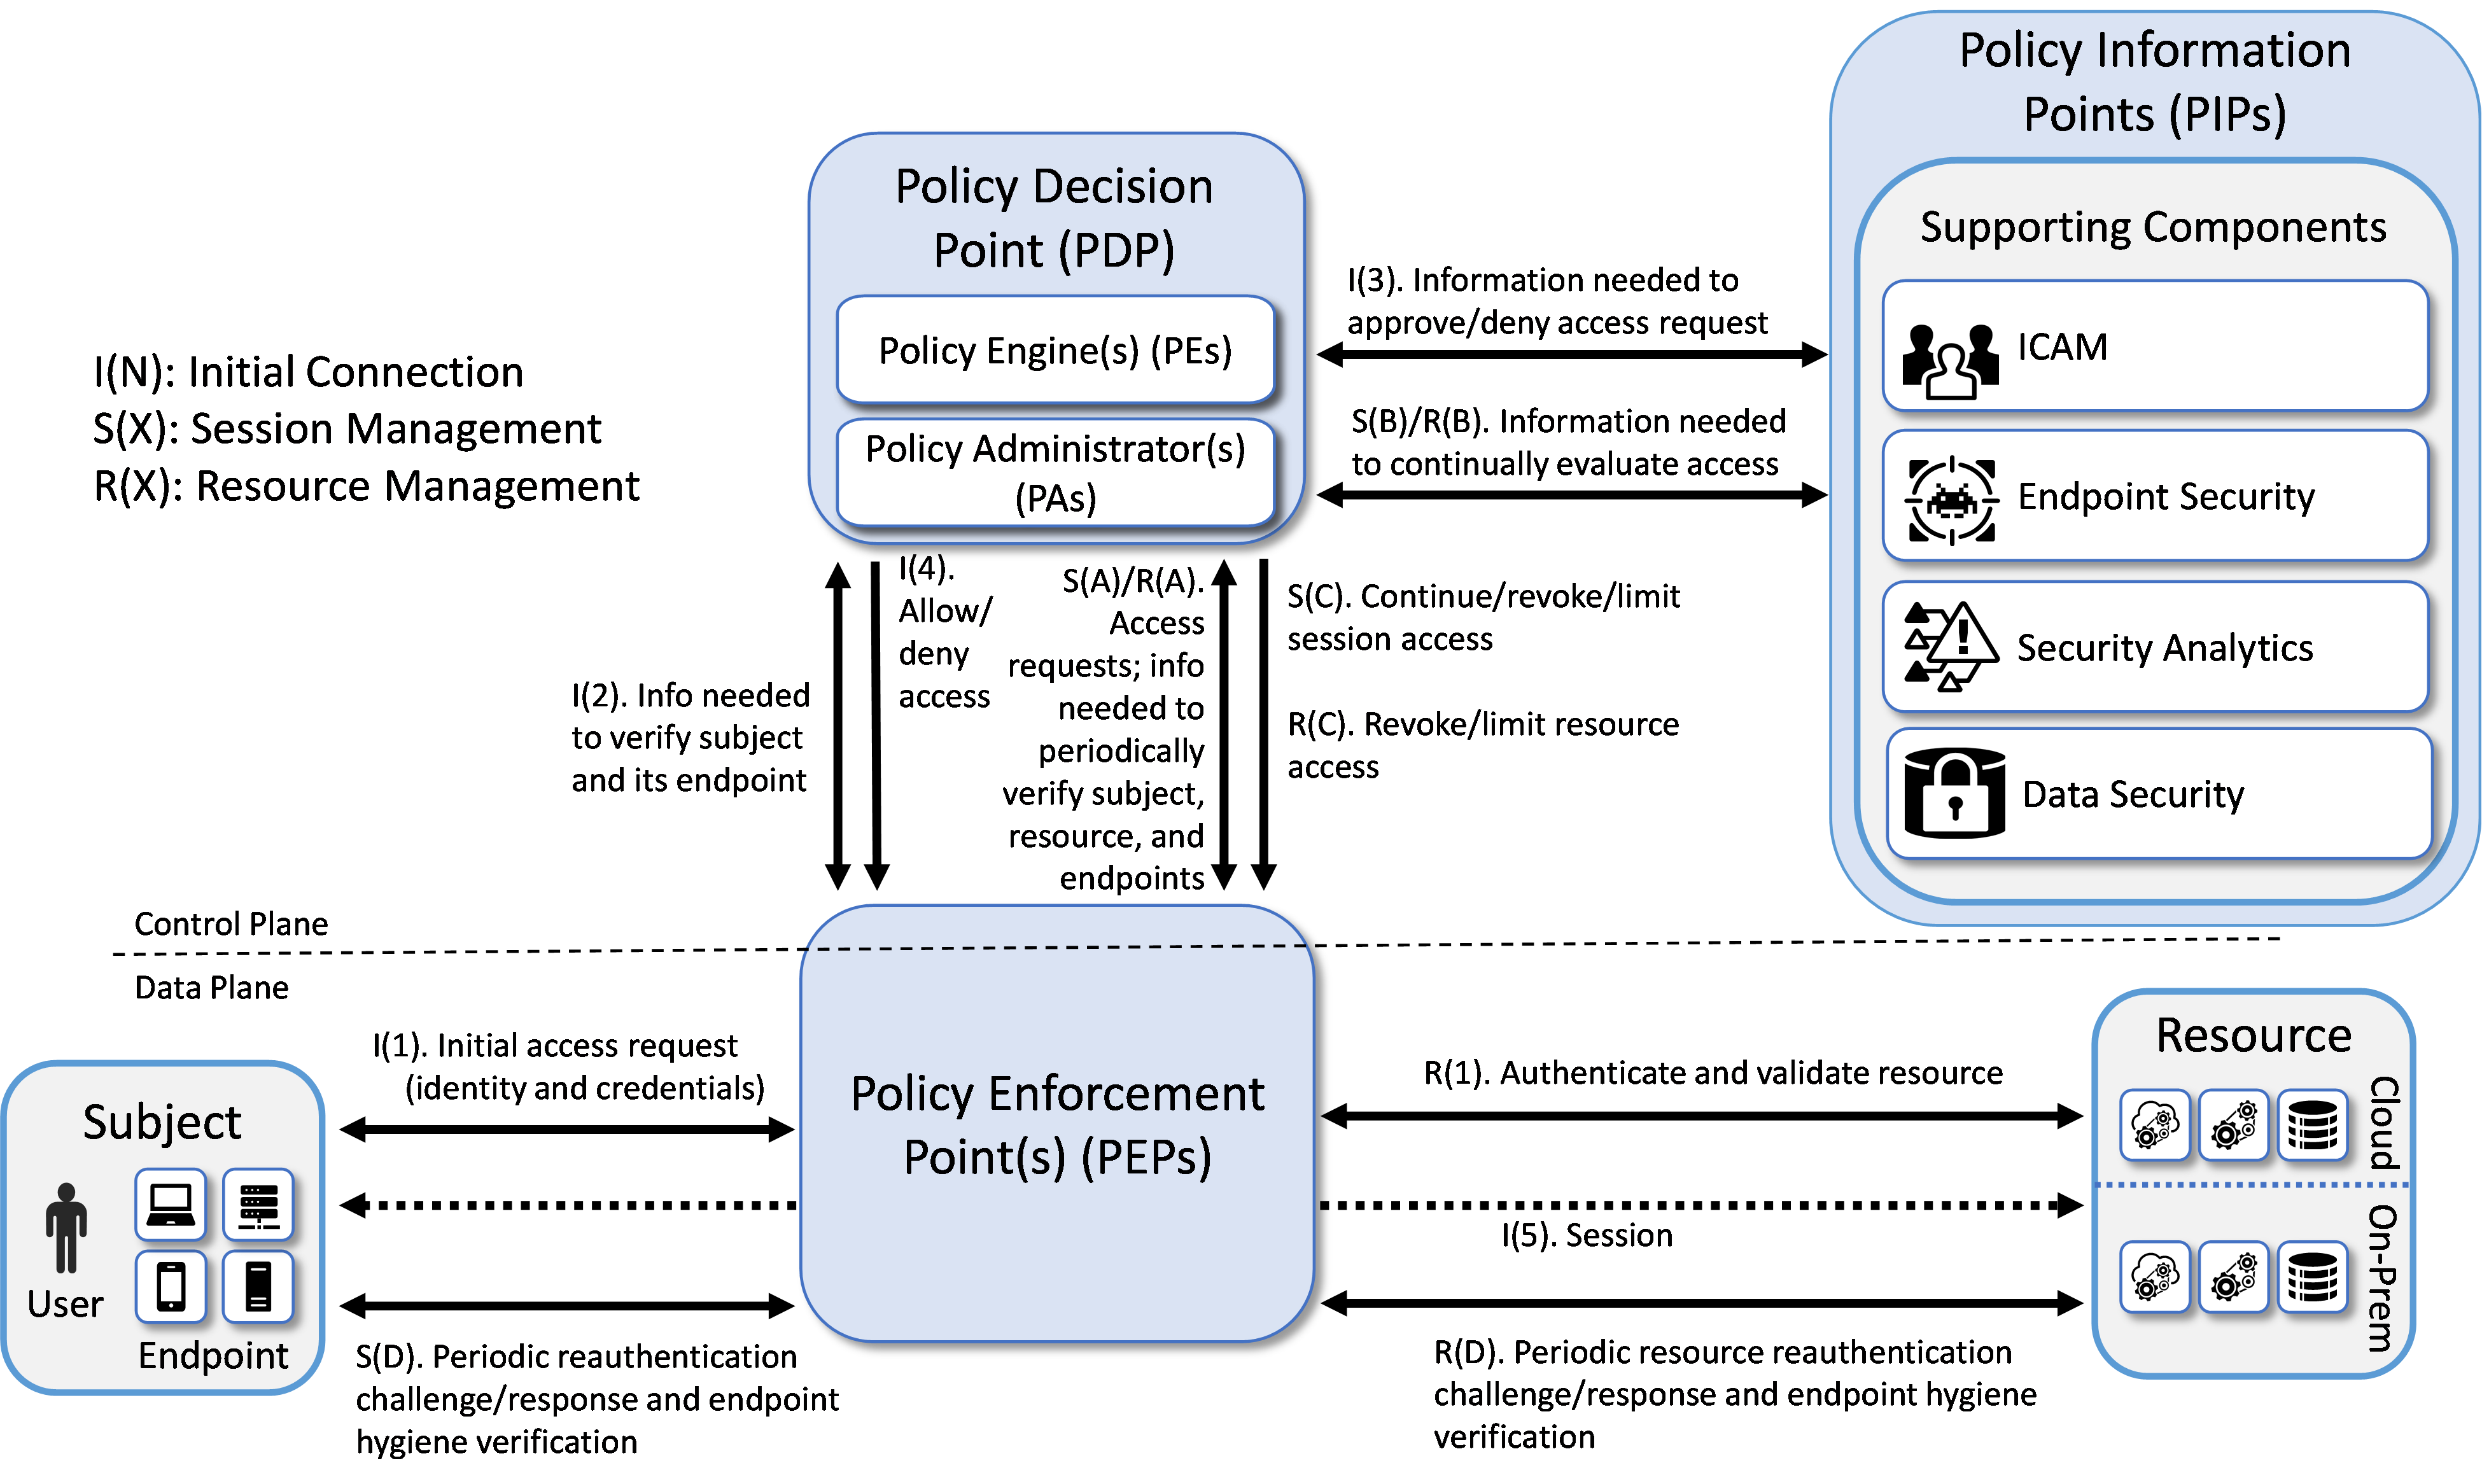
\includegraphics[width=0.35\textwidth,keepaspectratio]{gambar/NIST_Zero_Trust_Architecture.png}
    \hspace{0.3cm}
    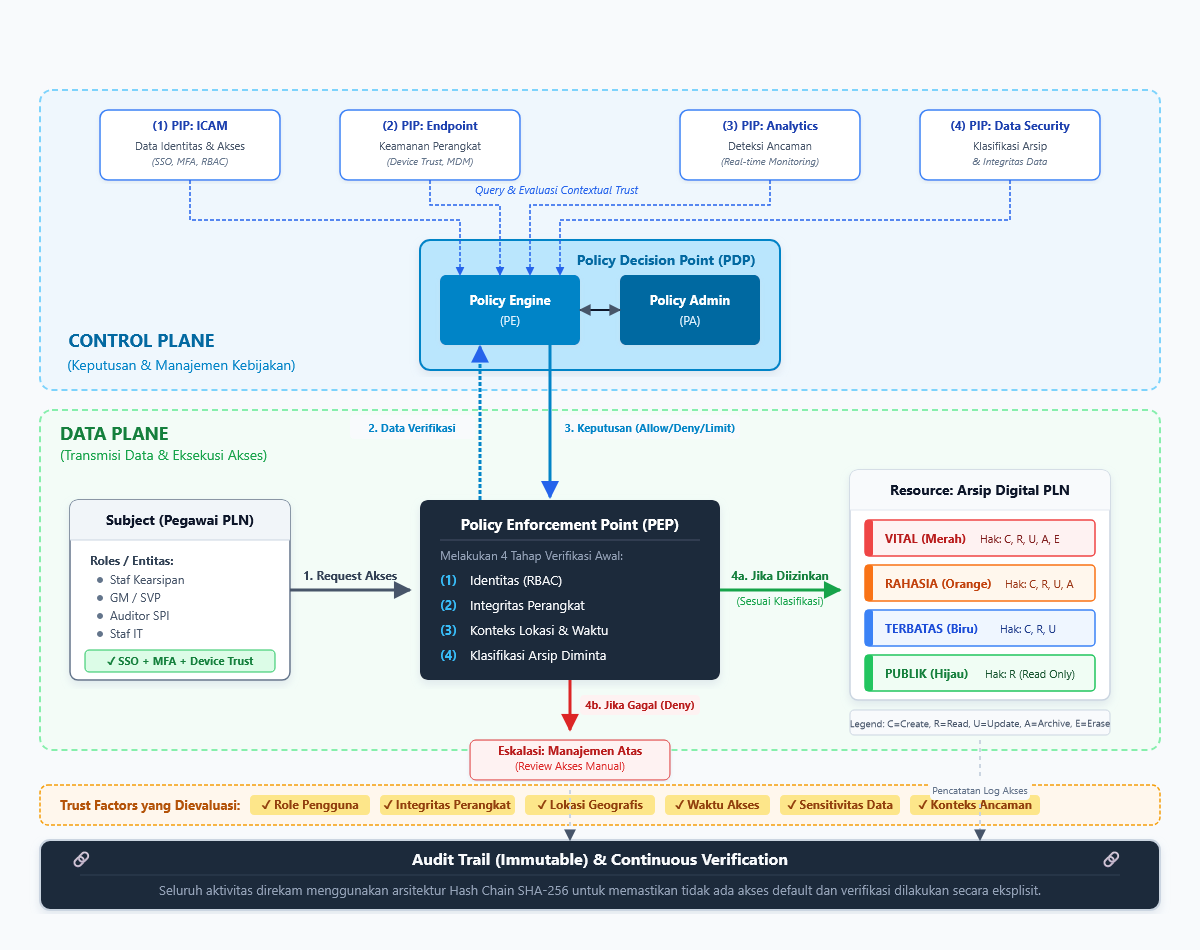
\includegraphics[width=0.35\textwidth,keepaspectratio]{gambar/nist.png}
    
    \vspace{0.1cm}
    {\tiny Sumber: NIST SP 800-207 \& SP 1800-35}
\end{frame}

% SLIDE 22: INTEGRASI GCG BUMN (TARIF)
\begin{frame}{Integrasi GCG BUMN: Prinsip TARIF}
    \vspace{0.1cm}
    \centering
    \scriptsize
    \begin{tabularx}{\textwidth}{@{} l X @{}}
        \toprule
        \textbf{Prinsip TARIF} & \textbf{Implementasi dalam Kebijakan Arsip} \\
        \midrule
        \rowcolor{rowalt}
        \textbf{Transparansi} & Audit trail dapat diakses Auditor Internal/Eksternal sesuai kewenangan \\
        \textbf{Akuntabilitas} & RACI digital jelas; setiap aksi terikat identitas \& TTE \\
        \rowcolor{rowalt}
        \textbf{Responsibilitas} & Kepatuhan PP 71/2019 \& Perka ANRI 6/2021 wajib diuji berkala \\
        \textbf{Independensi} & Unit Kearsipan berwenang tolak arsip tidak memenuhi standar metadata \\
        \rowcolor{rowalt}
        \textbf{Fairness} & Akses berbasis need-to-know, tidak diskriminatif, ada mekanisme banding \\
        \bottomrule
    \end{tabularx}
    
    \vspace{0.2cm}
    \begin{orangebox}[Manajemen Atas sebagai Penandatangan]
        \scriptsize Kebijakan yang tidak ditinjau secara berkala (minimal tahunan) akan menjadi usang dan kehilangan kekuatan hukumnya.
    \end{orangebox}
\end{frame}

% SLIDE 23: TEMPLATE KEBIJAKAN
\begin{frame}{Template Kerangka Kebijakan Keamanan Arsip}
    \vspace{0.1cm}
    \begin{columns}[T]
        \column{0.48\textwidth}
        \scriptsize
        \begin{premiumbox}[Klausul 1--3]
            \begin{itemize}
                \item \textbf{Ruang Lingkup} -- Seluruh arsip digital unit.
                \item \textbf{Kontrol Akses} -- RBAC, least privilege, provisioning.
                \item \textbf{Audit Trail} -- 14 field, immutable, retensi sesuai arsip.
            \end{itemize}
        \end{premiumbox}
        
        \column{0.48\textwidth}
        \scriptsize
        \begin{orangebox}[Klausul 4--6]
            \begin{itemize}
                \item \textbf{Backup \& Pemulihan} -- Strategi 3-2-1, RTO/RPO, simulasi 6 bulanan.
                \item \textbf{Peran \& Tanggung Jawab} -- RACI: Accountable = GM/SVP.
                \item \textbf{Kepatuhan \& Peninjauan} -- Audit internal, review tahunan.
            \end{itemize}
        \end{orangebox}
    \end{columns}
    
    \vspace{0.2cm}
    \begin{greenbox}[Insight]
        \scriptsize Kebijakan harus terintegrasi dengan ISMS organisasi (ISO 27001), bukan dokumen yang berdiri sendiri.
    \end{greenbox}
\end{frame}

% SLIDE 24: LANGKAH PERUMUSAN KEBIJAKAN
\begin{frame}{Langkah Perumusan Kebijakan}
    \vspace{0.2cm}
    \centering
    \begin{tikzpicture}[
        stepbox/.style={rectangle, rounded corners=4pt, draw=plnblue, fill=plnblue!5, minimum width=2.6cm, minimum height=1.4cm, align=center, font=\tiny\bfseries, line width=0.8pt},
        arrst/.style={-{Stealth[length=5pt]}, thick, plnblue}
    ]
        \node[stepbox] (s1) at (0,0) {Analisis\\Risiko};
        \node[stepbox] (s2) at (2.8,0) {Draf oleh\\Tim Lintas Fungsi};
        \node[stepbox] (s3) at (5.6,0) {Konsultasi\\Internal};
        \node[stepbox] (s4) at (8.4,0) {Pengesahan\\MA};
        \node[stepbox] (s5) at (11.2,0) {Sosialisasi\\\& Review};
        
        \draw[arrst] (s1) -- (s2);
        \draw[arrst] (s2) -- (s3);
        \draw[arrst] (s3) -- (s4);
        \draw[arrst] (s4) -- (s5);
    \end{tikzpicture}
    
    \vspace{0.3cm}
    \begin{premiumbox}[Peran Manajemen Atas]
        \small
        Mengesahkan kebijakan, menetapkan tanggal efektif, menunjuk penanggung jawab implementasi, \& memastikan review berkala minimal tahunan.
    \end{premiumbox}
\end{frame}

% SLIDE 25: OUTPUT PILAR 3
\begin{frame}{Output \& Workshop: Pilar 3 (Kebijakan ISMS)}
    \vspace{0.2cm}
    \begin{columns}[T]
        \column{0.48\textwidth}
        \begin{premiumbox}[Workshop 3 (30 Menit)]
            \scriptsize
            \begin{enumerate}
                \item Susun draf klausul kebijakan keamanan arsip (maks. 2 halaman).
                \item Petakan minimal 3 kontrol ISO 27001 yang relevan dengan unit Anda.
                \item Integrasikan 1 klausul pendukung prinsip TARIF.
            \end{enumerate}
        \end{premiumbox}
        
        \column{0.48\textwidth}
        \begin{greenbox}[Portofolio 3]
            \scriptsize
            \textbf{Rancangan Kebijakan Keamanan Arsip Terintegrasi ISMS}.\\[0.1cm]
            \textit{Kriteria:} 4.4.3 -- keselarasan ISO 27001, Zero Trust/Least Privilege, integrasi GCG BUMN.
        \end{greenbox}
    \end{columns}
\end{frame}

% ================================================================
%  BAGIAN IV: PILAR 4 -- BACKUP & DR
% ================================================================

\section{Pilar 4:\\Backup \& Disaster Recovery Terintegrasi}

% SLIDE 26: STRATEGI 3-2-1
\begin{frame}{Strategi Backup 3-2-1 untuk Arsip PLN}
    \centering
    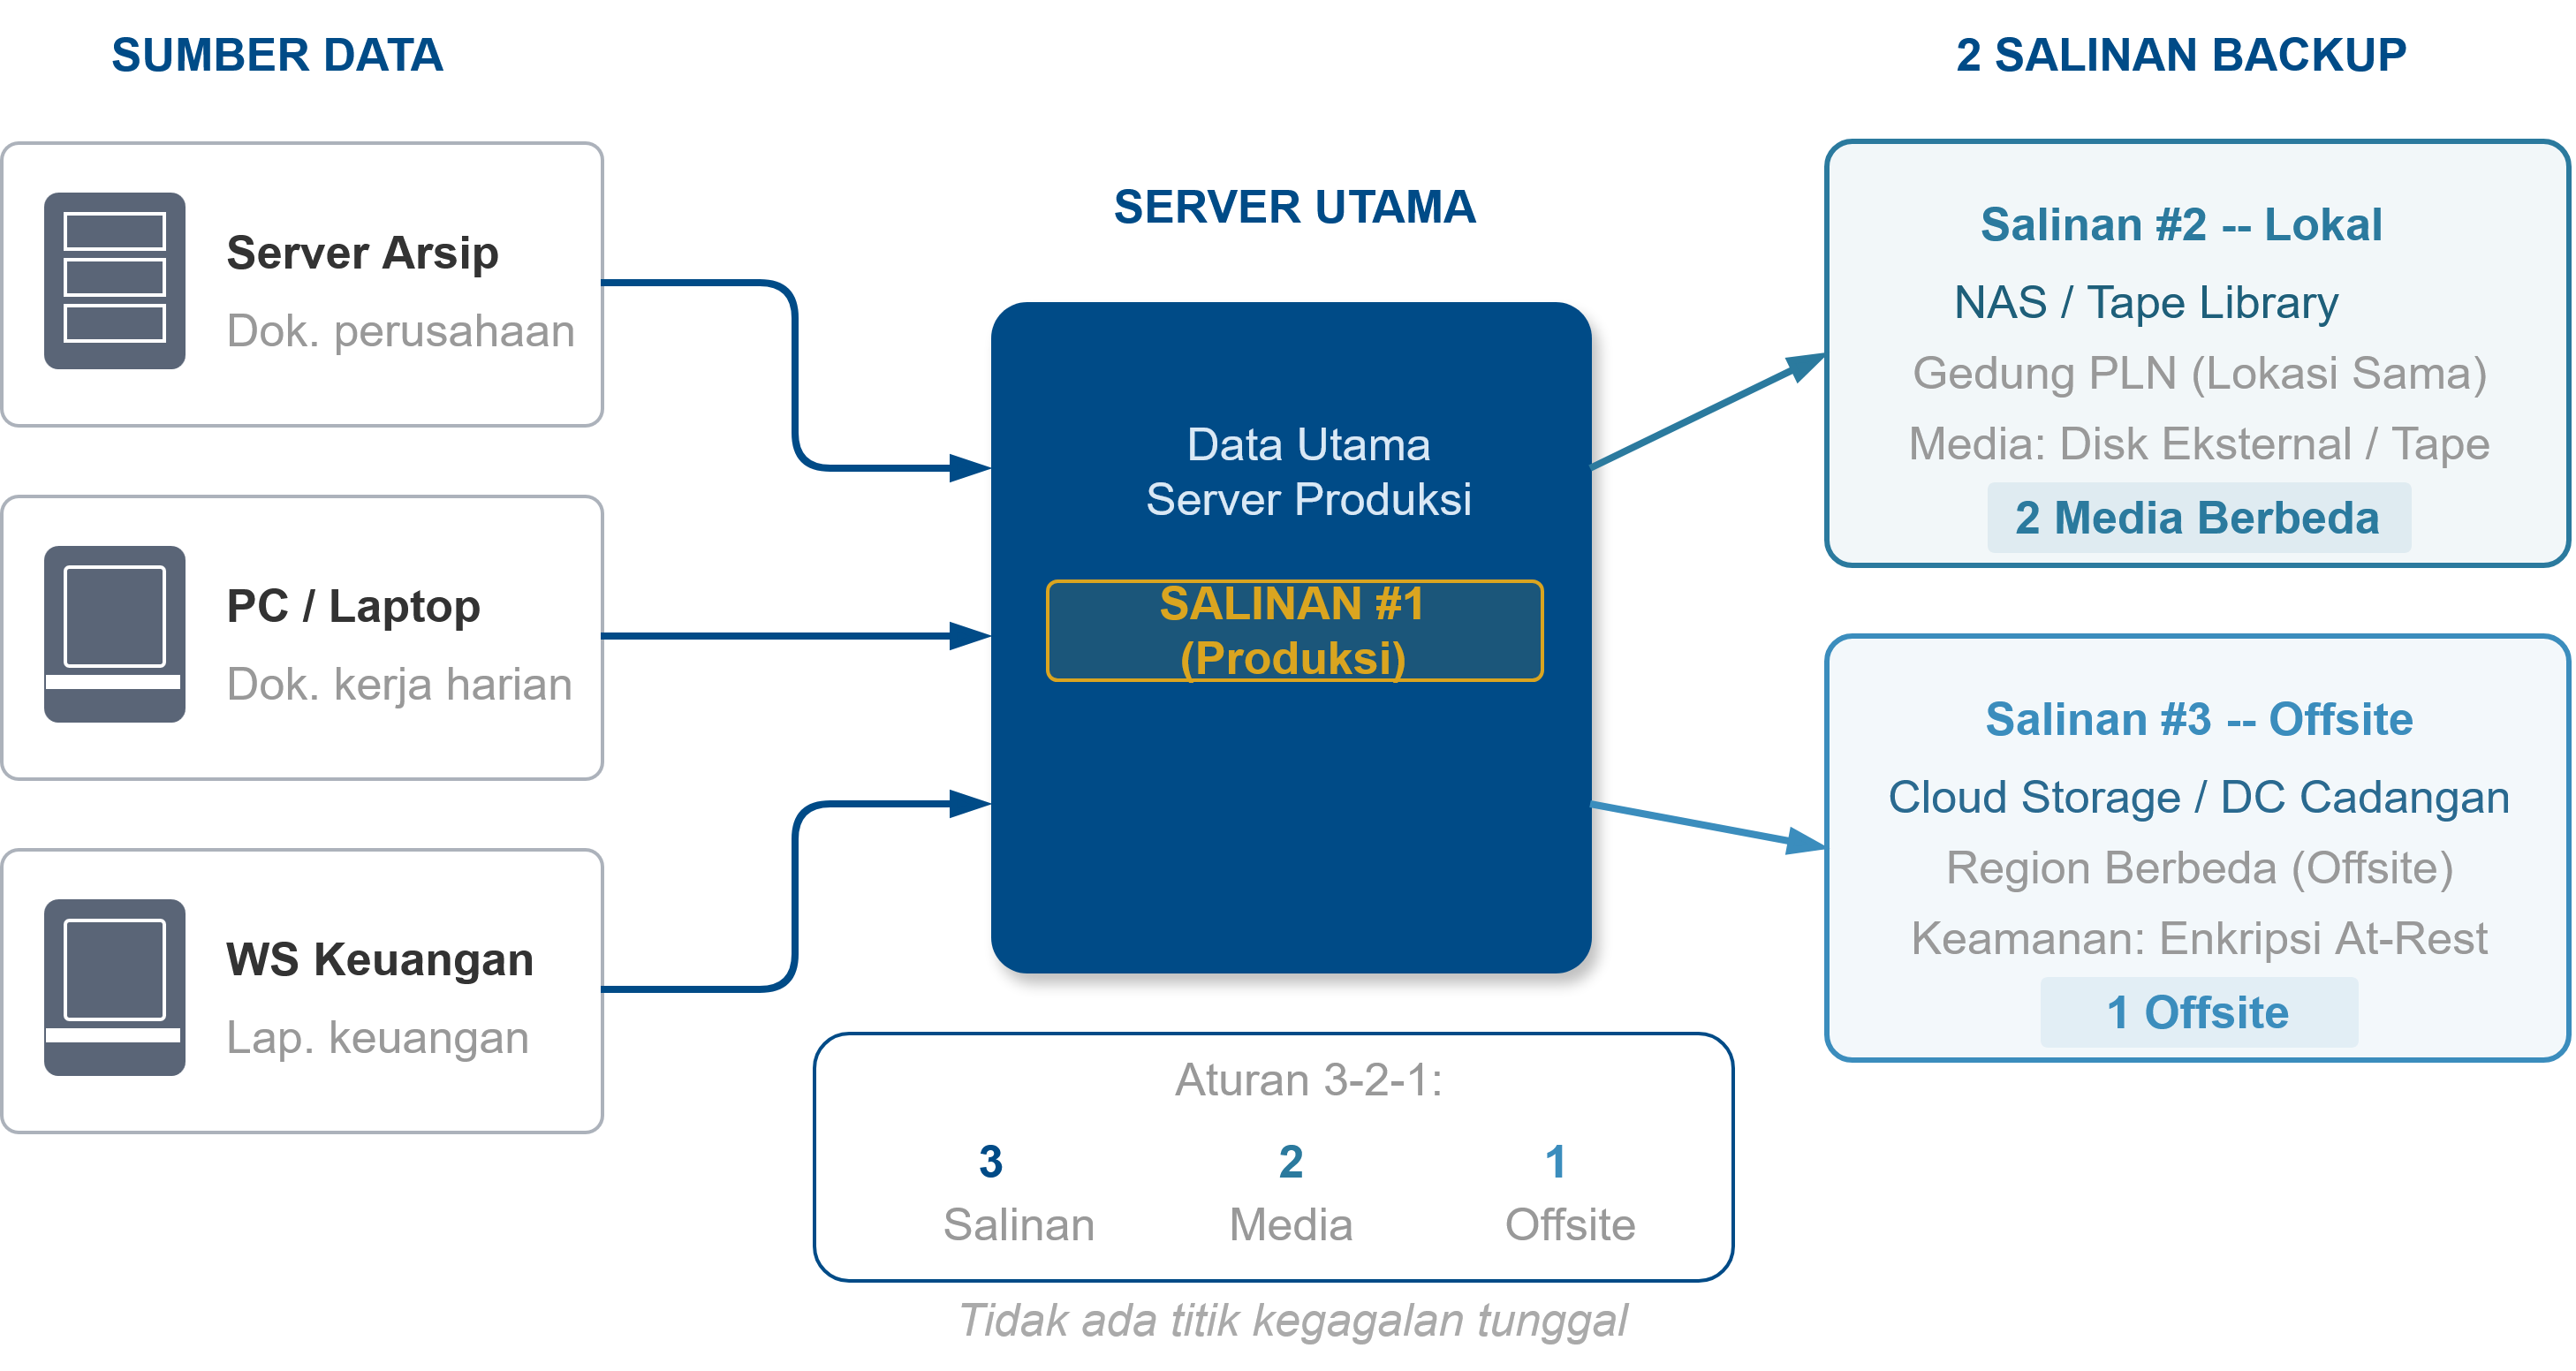
\includegraphics[width=0.85\textwidth,keepaspectratio]{321_rule.png}
    
    \vspace{0.2cm}
    \begin{columns}[T]
        \column{0.31\textwidth}
        \centering
        \stepicon{plnblue}{3} \\ \textbf{Salinan}\\
        \scriptsize Produksi + 2 backup
        
        \column{0.31\textwidth}
        \centering
        \stepicon{plncyan}{2} \\ \textbf{Media}\\
        \scriptsize NAS/Tape + Cloud/Offsite
        
        \column{0.31\textwidth}
        \centering
        \stepicon{plnorange}{1} \\ \textbf{Offsite}\\
        \scriptsize Lokasi geografis terpisah
    \end{columns}
\end{frame}

% SLIDE 27: RTO & RPO
\begin{frame}{RTO \& RPO: Target Pemulihan Berbasis Klasifikasi}
    \vspace{0.2cm}
    \begin{columns}[T]
        \column{0.48\textwidth}
        \centering
        \resizebox{0.95\textwidth}{!}{%
        \begin{tikzpicture}
            \definecolor{avail}{RGB}{26,58,92}
            \definecolor{disaster}{RGB}{192,57,43}
            \definecolor{recovered}{RGB}{39,174,96}
            \draw[avail, line width=2.5pt, -{Stealth[length=6pt]}] (0,3) -- (7.0,3);
            \draw[disaster, line width=2.5pt, dashed] (7.2,3) -- (10.0,3);
            \draw[avail, line width=2.5pt, -{Stealth[length=5pt]}] (10.2,3) -- (12.0,3);
            \node[font=\scriptsize\itshape, text=gray] at (11.5,2.5) {time};
            \draw[avail, line width=1.5pt] (1.5,2.7) -- (1.5,3.3);
            \node[font=\scriptsize\itshape, text=avail, anchor=north] at (1.5,2.65) {Backup};
            \draw[avail, line width=1.5pt] (3.0,2.7) -- (3.0,3.3);
            \node[font=\scriptsize\itshape, text=avail, anchor=north] at (3.0,2.65) {Backup};
            \draw[avail, line width=1.5pt] (5.0,2.7) -- (5.0,3.3);
            \node[font=\scriptsize\itshape, text=avail, anchor=south] at (5.0,3.35) {Recovery Point};
            \draw[disaster, line width=2pt] (7.2,2.5) -- (7.2,3.3);
            \fill[disaster] (7.0,4.0) -- (7.3,3.5) -- (7.1,3.5) -- (7.4,2.8) -- (7.1,3.15) -- (7.3,3.15) -- cycle;
            \node[font=\small\bfseries\itshape, text=disaster] at (7.2,4.25) {Disaster};
            \draw[recovered, line width=2pt] (10.2,2.7) -- (10.2,3.3);
            \node[font=\scriptsize\itshape, text=recovered, anchor=south] at (10.2,3.35) {Recovered};
            \draw[avail, line width=1.2pt] (3.0,1.4) -- (5.0,1.4);
            \draw[avail, line width=1.2pt] (3.0,1.1) -- (3.0,1.7);
            \draw[avail, line width=1.2pt] (5.0,1.1) -- (5.0,1.7);
            \fill[avail] (3.15,1.4) -- (3.0,1.2) -- (3.0,1.6) -- cycle;
            \fill[avail] (4.85,1.4) -- (5.0,1.2) -- (5.0,1.6) -- cycle;
            \node[avail, font=\small\bfseries] at (4.0,1.0) {RPO};
            \draw[disaster, line width=1.2pt, dashed] (7.2,0.0) -- (10.2,0.0);
            \draw[disaster, line width=1.2pt] (7.2,-0.3) -- (7.2,0.3);
            \draw[disaster, line width=1.2pt] (10.2,-0.3) -- (10.2,0.3);
            \fill[disaster] (7.35,0.0) -- (7.2,-0.2) -- (7.2,0.2) -- cycle;
            \fill[disaster] (10.05,0.0) -- (10.2,-0.2) -- (10.2,0.2) -- cycle;
            \node[disaster, font=\small\bfseries] at (8.7,-0.4) {RTO};
        \end{tikzpicture}%
        }
        
        \column{0.48\textwidth}
        \scriptsize
        \begin{tabularx}{\textwidth}{@{} >{\raggedright\arraybackslash}p{1.8cm} >{\centering\arraybackslash}p{1.6cm} >{\centering\arraybackslash}p{1.6cm} X @{}}
            \toprule
            \rowcolor{rowhead}
            \textcolor{white}{\textbf{Klasif.}} & \textcolor{white}{\textbf{RTO}} & \textcolor{white}{\textbf{RPO}} & \textcolor{white}{\textbf{Strategi}} \\
            \midrule
            \rowcolor{rowalt}
            Vital & $<$4 jam & $<$1 jam & Mirror site, failover otomatis \\
            Rahasia & $<$12 jam & $<$4 jam & Backup harian terenkripsi \\
            \rowcolor{rowalt}
            Internal & $<$24 jam & $<$12 jam & Backup mingguan, cold storage \\
            \bottomrule
        \end{tabularx}
        
        \vspace{0.2cm}
        \begin{greenbox}[Keputusan Bisnis]
            \scriptsize RTO/RPO = keputusan strategis, bukan teknis semata. Proporsional dengan klasifikasi \& anggaran.
        \end{greenbox}
    \end{columns}
\end{frame}

% SLIDE 28: BCP LIFECYCLE
\begin{frame}{Business Continuity Plan (BCP): Siklus Hidup ISO 22301}
    \centering
    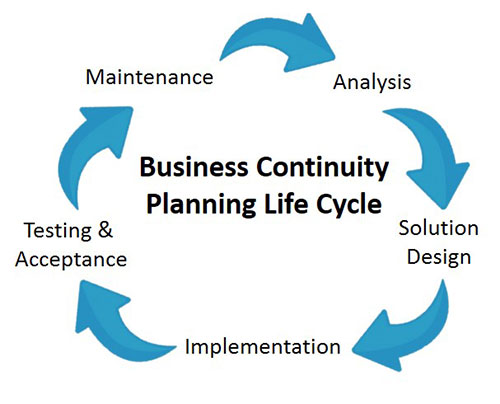
\includegraphics[width=0.38\textwidth,keepaspectratio]{gambar/BCP_Lifecycle_Custom.png}
    
    \vspace{0.08cm}
    \begin{columns}[T]
        \column{0.48\textwidth}
        \begin{premiumbox}[5 Fase Iteratif]
            \tiny
            \begin{enumerate}
                \item \textbf{Analysis} -- BIA \& penilaian risiko.
                \item \textbf{Solution Design} -- Strategi pemulihan.
                \item \textbf{Implementation} -- SOP, tim, infrastruktur.
            \end{enumerate}
        \end{premiumbox}
        
        \column{0.48\textwidth}
        \begin{orangebox}[Pemeliharaan]
            \tiny
            \begin{enumerate}\setcounter{enumi}{3}
                \item \textbf{Testing \& Acceptance} -- Simulasi \& validasi.
                \item \textbf{Maintenance} -- Update berkala.
            \end{enumerate}
            \vspace{0.05cm}
            \textbf{\tiny Simulasi minimal 6 bulan sekali!}
        \end{orangebox}
    \end{columns}
\end{frame}

% SLIDE 29: LANGKAH PERANCANGAN DR
\begin{frame}{Langkah Perancangan Sistem Backup/DR}
    \vspace{0.2cm}
    \begin{columns}[T]
        \column{0.48\textwidth}
        \begin{premiumbox}[Tata Kelola]
            \scriptsize
            \begin{enumerate}
                \item \textbf{BIA} -- Identifikasi arsip vital \& estimasi dampak.
                \item \textbf{Tetapkan RTO/RPO} -- Realistis \& proporsional anggaran.
                \item \textbf{Strategi 3-2-1} -- Setujui alokasi anggaran (cloud, offsite, enkripsi).
            \end{enumerate}
        \end{premiumbox}
        
        \column{0.48\textwidth}
        \begin{orangebox}[Kesiapan Organisasi]
            \scriptsize
            \begin{enumerate}\setcounter{enumi}{3}
                \item \textbf{Prosedur Fallback} -- Jika sistem lumpuh $>$4 jam, bagaimana unit beroperasi?
                \item \textbf{Simulasi Berkala} -- Minimal 6 bulanan; MA terima laporan hasil.
            \end{enumerate}
        \end{orangebox}
    \end{columns}
    
    \vspace{0.2cm}
    \begin{center}
        \textcolor{plnblue}{\scriptsize\textit{Pertanyaan Kunci: ``Jika arsip vital musnah besok, berapa kerugian finansial \& apakah kita siap hadapi regulator?''}}
    \end{center}
\end{frame}

% SLIDE 30: OUTPUT PILAR 4
\begin{frame}{Output \& Workshop: Pilar 4 (Backup \& DR)}
    \vspace{0.2cm}
    \begin{columns}[T]
        \column{0.48\textwidth}
        \begin{premiumbox}[Workshop 4 (30 Menit)]
            \scriptsize
            \begin{enumerate}
                \item Tentukan klasifikasi arsip vital di unit Anda.
                \item Tetapkan target RTO/RPO realistis.
                \item Rancang jadwal backup \& skenario simulasi 6 bulanan.
            \end{enumerate}
        \end{premiumbox}
        
        \column{0.48\textwidth}
        \begin{greenbox}[Portofolio 4]
            \scriptsize
            \textbf{Matriks RTO/RPO} + Rencana Backup \& DR.\\[0.1cm]
            \textit{Kriteria:} 4.4.4 -- kesesuaian 3-2-1, target realistis, prosedur fallback/simulasi.
        \end{greenbox}
    \end{columns}
\end{frame}


% ================================================================
%  BAGIAN V: STUDI KASUS INTEGRATIF
% ================================================================

\section{Studi Kasus:\\Insiden Kebocoran Arsip Kontrak}

% SLIDE 31: SKENARIO
\begin{frame}{Skenario Insiden}
    \vspace{0.2cm}
    \begin{orangebox}[Kejadian]
        \small
        Senin pukul 08.00, Manajer Keuangan Unit Bisnis PLN XYZ menemukan bahwa dokumen kontrak jangka panjang dengan vendor strategis telah \textbf{diunduh oleh 3 orang tidak berwenang} pada Jumat malam pukul 23.45.
        \begin{itemize}
            \item Status dokumen: \textbf{Rahasia}.
            \item Deteksi baru terjadi setelah \textbf{2,5 hari}.
            \item Staf administrasi memeriksa log \& menemukan anomali secara kebetulan.
        \end{itemize}
    \end{orangebox}
    
    \begin{premiumbox}[Pertanyaan Strategis]
        \small
        Apakah keempat pilar keamanan kita berfungsi? Di mana letak kelemahan sistemiknya?
    \end{premiumbox}
\end{frame}

% SLIDE 32: ANALISIS PILAR 1 & 2
\begin{frame}{Analisis: Pilar 1 (RBAC) \& Pilar 2 (Audit Trail)}
    \vspace{0.2cm}
    \begin{columns}[T]
        \column{0.48\textwidth}
        \begin{premiumbox}[Pilar 1: RBAC]
            \scriptsize
            \textbf{Temuan:} Ketiga pelaku berperan Staf Administrasi --- seharusnya hanya Read, bukan Export.
            \vspace{0.1cm}
            \begin{itemize}
                \item \textcolor{red}{Akar:} Matriks RBAC tidak membedakan View vs Export.
                \item \textcolor{plnblue}{Tindakan:} Revisi matriks; pisahkan hak. Export Rahasia hanya via prosedur darurat.
            \end{itemize}
        \end{premiumbox}
        
        \column{0.48\textwidth}
        \begin{orangebox}[Pilar 2: Audit Trail]
            \scriptsize
            \textbf{Temuan Positif:} Aksi download tercatat lengkap (who, when, where).
            \vspace{0.1cm}
            \begin{itemize}
                \item \textcolor{red}{Akar:} Tidak ada alert otomatis untuk ekspor di luar jam kerja (23.45 = mencurigakan).
                \item \textcolor{plnblue}{Tindakan:} Tetapkan aturan SIEM: alert otomatis untuk event kritis.
            \end{itemize}
        \end{orangebox}
    \end{columns}
\end{frame}

% SLIDE 33: ANALISIS PILAR 3 & 4
\begin{frame}{Analisis: Pilar 3 (Kebijakan) \& Pilar 4 (Backup/DR)}
    \vspace{0.2cm}
    \begin{columns}[T]
        \column{0.48\textwidth}
        \begin{premiumbox}[Pilar 3: Kebijakan ISMS]
            \scriptsize
            \textbf{Temuan:} Kebijakan tidak mengatur spesifik ekspor terkontrol untuk arsip Rahasia.
            \vspace{0.1cm}
            \begin{itemize}
                \item \textcolor{red}{Akar:} Kebijakan belum direview 18 bulan (melampaui siklus tahunan ISO 27001).
                \item \textcolor{plnblue}{Tindakan:} Revisi klausul ekspor, tetapkan jadwal review, libatkan stakeholders.
            \end{itemize}
        \end{premiumbox}
        
        \column{0.48\textwidth}
        \begin{orangebox}[Pilar 4: Backup/DR]
            \scriptsize
            \textbf{Temuan Positif:} Arsip masih tersedia --- integritas data tidak terganggu.
            \vspace{0.1cm}
            \begin{itemize}
                \item \textcolor{red}{Pertanyaan Kritis:} Jika ini \textit{ransomware}, berapa lama pemulihan? Apakah backup terpisah dari jaringan produksi?
                \item \textcolor{plnblue}{Tindakan:} Verifikasi 3-2-1 \& simulasi pemulihan $<$6 bulan terakhir.
            \end{itemize}
        \end{orangebox}
    \end{columns}
\end{frame}

% SLIDE 34: PELAJARAN
\begin{frame}{Pelajaran untuk Manajemen Atas}
    \vspace{0.2cm}
    \begin{premiumbox}[Sistem Terintegrasi, Bukan Parsial]
        \small
        Kelemahan pada satu pilar akan menetralisasi kekuatan pilar lainnya:
        \begin{itemize}
            \item RBAC tidak detail (Pilar 1) $\rightarrow$ celah akses.
            \item Tanpa pemantauan aktif (Pilar 2) $\rightarrow$ pelanggaran terlambat terdeteksi.
            \item Tanpa kebijakan spesifik (Pilar 3) $\rightarrow$ tidak ada dasar hukum tindak lanjut.
            \item Tanpa backup teruji (Pilar 4) $\rightarrow$ dampak besar tidak dapat dipulihkan.
        \end{itemize}
    \end{premiumbox}
    
    \vspace{0.2cm}
    \begin{greenbox}[Refleksi Mandiri]
        \small
        Identifikasi minimal \textbf{2 celah keamanan} yang berpotensi terjadi di unit Anda. Tentukan tindakan perbaikan per pilar, PIC, \& timeline.
    \end{greenbox}
\end{frame}

% ================================================================
%  BAGIAN VI: VALIDASI & PENUTUP
% ================================================================

\section{Validasi, Portofolio \& Executive Tollgate}

% SLIDE 35: PEMETAAN PORTOFOLIO
\begin{frame}{Pemetaan Portofolio \& Kriteria Penilaian}
    \vspace{0.1cm}
    \centering
    \scriptsize
    \begin{tabularx}{\textwidth}{@{} >{\centering\arraybackslash}p{1cm} >{\raggedright\arraybackslash}p{3cm} X >{\centering\arraybackslash}p{1cm} @{}}
        \toprule
        \rowcolor{rowhead}
        \textcolor{white}{\textbf{Pilar}} & \textcolor{white}{\textbf{Target Kompetensi}} & \textcolor{white}{\textbf{Portofolio Wajib}} & \textcolor{white}{\textbf{Bobot}} \\
        \midrule
        \rowcolor{rowalt}
        1 & RBAC terintegrasi dengan kepegawaian & Matriks RBAC + Prosedur Akses & 25\% \\
        2 & Audit trail otomatis & Alur Audit + Template 14 Field & 25\% \\
        \rowcolor{rowalt}
        3 & Kebijakan terintegrasi ISMS & Rancangan Kebijakan Keamanan & 25\% \\
        4 & Backup \& DR terintegrasi & Matriks RTO/RPO + Rencana DR & 25\% \\
        \bottomrule
    \end{tabularx}
    
    \vspace{0.3cm}
    \begin{columns}[T]
        \column{0.48\textwidth}
        \begin{premiumbox}[Kriteria Kelulusan]
            \scriptsize
            \begin{itemize}
                \item Skor portofolio $\geq$ 70/100
                \item Post-test $\geq$ 65
                \item Komitmen tindak lanjut tertulis
            \end{itemize}
        \end{premiumbox}
        
        \column{0.48\textwidth}
        \begin{orangebox}[Pengingat]
            \scriptsize Keempat portofolio bersifat \textbf{kumulatif \& terintegrasi}. Pilar 1 menjadi input Pilar 2, yang menjadi input Pilar 3, dan seterusnya.
        \end{orangebox}
    \end{columns}
\end{frame}

% SLIDE 36: EXECUTIVE TOLLGATE
\begin{frame}{Executive Tollgate: 4 Gate Sebelum Implementasi}
    \vspace{0.2cm}
    \begin{columns}[T]
        \column{0.35\textwidth}
        \centering
        \begin{tikzpicture}[
            gate/.style={circle, draw=plnblue, fill=white, thick, minimum size=0.9cm, font=\bfseries\small},
            line/.style={ultra thick, plnblue!30}
        ]
            \draw[line] (0, 3.2) -- (0, -0.8);
            \node[gate, fill=plnblue!10] (g1) at (0, 2.8) {1};
            \node[gate, fill=plncyan!10, draw=plncyan] (g2) at (0, 1.6) {2};
            \node[gate, fill=plnorange!10, draw=plnorange] (g3) at (0, 0.4) {3};
            \node[gate, fill=plngreen!10, draw=plngreen] (g4) at (0, -0.8) {4};
            \node[anchor=west, font=\scriptsize] at (0.7, 2.8) {Legal Compliance};
            \node[anchor=west, font=\scriptsize] at (0.7, 1.6) {Data Integrity};
            \node[anchor=west, font=\scriptsize] at (0.7, 0.4) {Operational Value};
            \node[anchor=west, font=\scriptsize] at (0.7, -0.8) {Scalability};
        \end{tikzpicture}
        
        \column{0.62\textwidth}
        \begin{premiumbox}[Kriteria Verifikasi]
            \scriptsize
            \begin{itemize}
                \item[\textbf{G1}] Selaras PP 71/2019 \& Perka ANRI 6/2021?
                \item[\textbf{G2}] Jamin keaslian via Hash + TTE + Audit Immutable?
                \item[\textbf{G3}] Mitigasi risiko terkuantifikasi (downtime $\downarrow$, temuan audit $\rightarrow$0)?
                \item[\textbf{G4}] Infrastruktur \& prosedur siap diskalakan jangka panjang?
            \end{itemize}
        \end{premiumbox}
        \vspace{0.1cm}
        \begin{orangebox}[Aturan Emas]
            \scriptsize Jika \textbf{salah satu gate} bernilai ``No'', lakukan perancangan ulang sebelum diajukan ke Komite Tata Kelola.
        \end{orangebox}
    \end{columns}
\end{frame}

% SLIDE 37: REFLEKSI & KOMITMEN
\begin{frame}{Refleksi \& Komitmen Tindak Lanjut}
    \vspace{0.2cm}
    \begin{premiumbox}[Pertanyaan Refleksi Mandiri]
        \small
        \begin{enumerate}
            \item Apa \textbf{1 celah keamanan} paling kritis di unit Anda saat ini?
            \item Siapa \textbf{pemangku kepentingan kunci} (IT, GCG, Legal, SPI) yang harus dilibatkan?
            \item Berapa \textbf{timeline realistis} untuk merampungkan 4 portofolio ini?
        \end{enumerate}
    \end{premiumbox}
    
    \vspace{0.2cm}
    \begin{orangebox}[Lembar Komitmen 30 Hari]
        \small
        Saya, \underline{\hspace{2.5cm}}, menyatakan akan menginisiasi perbaikan keamanan arsip pada proses \underline{\hspace{2.5cm}} dengan target KPI \underline{\hspace{2cm}} dan melaporkan hasil kepada \underline{\hspace{2.5cm}} paling lambat tanggal~\underline{\hspace{2cm}}.
    \end{orangebox}
\end{frame}

% SLIDE 38: CLOSING
\begin{frame}{}
    \vspace{0.5cm}
    \begin{center}
        \huge \textcolor{plnblue}{\textbf{TERIMA KASIH}}\\[0.3cm]
        \large Mari Menuju Tata Kelola Arsip yang Aman, Terlacak, \& Tahan Audit!\\[0.6cm]
        \normalsize \textit{``Keamanan hari ini untuk keandalan hari esok.''}
    \end{center}
    \vspace{0.4cm}
    \begin{center}
        \begin{minipage}{0.65\textwidth}
            \begin{greenbox}[Langkah Selanjutnya]
                \scriptsize
                \begin{itemize}
                    \item Kerjakan \textbf{Post-Test} (10 soal)
                    \item Kumpulkan \textbf{4 Portofolio} sesuai rubrik penilaian
                    \item Jadwalkan \textbf{Peer Review} antar unit
                    \item Gunakan hasil sebagai acuan \textbf{Rencana Peningkatan Tahunan}
                \end{itemize}
            \end{greenbox}
        \end{minipage}
    \end{center}
\end{frame}

\end{document}
